\documentclass[a4paper]{article}

% You can change the parameters: here are the available options:
% - a4paper
% - fancysections
% - notitlepage or titlepage
% - onside or twoside for single-sided or double-sided printing
% - sectionmark
% - chaptermark
% - pagenumber
% When in doubt, the documentation can be found at:
% https://gitlab.binets.fr/typographix/polytechnique/-/blob/master/source/polytechnique.pdf

\usepackage[a4paper, sectionmark, pagenumber, chaptermark, notitlepage]{polytechnique}
\usepackage[english]{babel}
\usepackage[T1]{fontenc}
\usepackage{blindtext}
\usepackage[hidelinks]{hyperref}
\usepackage{amsmath, amssymb}
\usepackage{abstract}
\usepackage{booktabs}
\usepackage{ocgx2}      % For creating PDF layers (OCGs)
\usepackage{hyperref}
\usepackage{ragged2e}
\usepackage{float}

\usepackage{xcolor}
\usepackage{subcaption}
\usepackage{multirow}
\newsavebox{\mycomparisonboxtable}
\usepackage{tikz}
\usepackage{graphicx}
\usepackage{array}
\usepackage{booktabs}
\usepackage{caption}
\usepackage{amsmath}
\usepackage{dashbox} % For dashed boxes (alternatively use TikZ)


\definecolor{goodgreen}{rgb}{0.1, 0.6, 0.1}
\definecolor{badred}{rgb}{0.8, 0.1, 0.1}

\usetikzlibrary{positioning, shapes.geometric, arrows.meta}
\tikzset{
  block/.style={rectangle, draw=black, fill=blue!10, rounded corners, align=center, minimum width=2.8cm, minimum height=1.4cm},
  head/.style={rectangle, draw=black, fill=green!15, rounded corners, align=center, minimum width=3.2cm, minimum height=1.6cm},
  output/.style={rectangle, draw=black, fill=orange!25, rounded corners, align=center, minimum width=2.5cm, minimum height=1.4cm},
  arrow/.style={thick, -{Latex[length=3mm]}},
}


\newcommand{\code}[1]{%
    \mbox{\ttfamily%
        \detokenize{#1}%
    }%
}

\newcommand{\resultat}[1]{%
    \quad \rightsquigarrow \quad #1%
}

\author{Ayoub Agouzoul \\ Georgii Kuznetsov \\ Georgy Salakhutdinov}
\title{Zero-shot nutrition estimation}
\subtitle{Leveraging Deep Neural Networks for Automated Food Analysis}

\begin{document}
    \maketitle

    \begin{abstract}
        \noindent Keeping track of our food intake can still feel like a chore, even with so many nutrition apps available today. This project explores a potential solution through Machine Learning. We frame this challenge as a multi-output regression task. Given an RGB image of a plated dish, we want to predict its total weight together with calories, fat, carbs, and protein. The Nutrition5K dataset from Google Research has been utilized for training. This paper makes 3 contributions. Firstly, we present our data pipeline, which involves cleaning, segmentation, and a Principal Component Analysis (PCA) video frame extraction strategy. Secondly, we present our model WeightCNN that has been trained to predict weight with 18.7\% relative MAE. Finally, we present a family of relative-macro models that have been trained to estimate macronutrient percentages. These models are then combined with WeightCNN to obtain the full calorie and macronutrient prediction from a single photo.  
    \end{abstract}	

    \vfill

    \paragraph*{Acknowledgements}
    \noindent We would like to express our sincere gratitude to Professor Jesse Read and Professor Adrien Ehrhardt, for their invaluable guidance, and encouragement throughout the course of this project.

    
    \clearpage
    
    \tableofcontents
    \clearpage
    
	\section{Introduction} 
        \subsection{Problem Definition, Strategy and Metrics}
        \label{sec:metrics}
        With growing attention brought to ML and latest improvements in the field, more and more problems that seemed unresolvable before now can be solved. One of these tasks is estimating nutrition of the meal by taking a picture of it. This is a highly researched topic and demand for solution is insanely high. In general the problem is quite sophisticated, because even the companies themselves are allowed to have 20\% marginal error for calories estimation of their products. Many datasets, like \textit{Open Food Facts} \cite{openfoodfacts} exploit these errors, except \textit{Nutrition5k} \cite{thames2021nutrition5k} which seems to resolve this issue by manual labeling with professional nutritionists.
        
        We made an attempt to solve the limited task as well of trying to predict calories, fats, carbs and proteins by a picture of the meal. One of our inspirations of the methodology \cite{thames2021nutrition5k} is that we will not predict absolute values, but split the task in two - predicting the weight of the model and predicting the relative values per 100g. 
        We employed standard regression metrics to assess segmentation impact:
        \begin{itemize}
            \item \textbf{Mean Absolute Error (MAE):} $\text{MAE} = \frac{1}{N}\sum_{i=1}^N |y_i - \hat{y}_i|$
            \item \textbf{Relative MAE:} $\text{MAE}_{\%} = \frac{\text{MAE}}{\bar{y}} \times 100\%$
            \item \textbf{Root Mean Square Error (RMSE):} $\text{RMSE} = \sqrt{\frac{1}{N}\sum_{i=1}^N (y_i - \hat{y}_i)^2}$
            \item \textbf{Coefficient of Determination:} $R^2 = 1 - \frac{\sum_{i=1}^N(y_i - \hat{y}_i)^2}{\sum_{i=1}^N(y_i - \bar{y})^2}$
        \end{itemize}

        \section{Data Exploration and Preprocessing}
        \subsection{Dataset: Nutrition5K}
            The Nutrition5K dataset \cite{thames2021nutrition5k} is a comprehensive collection of realistic dishes from Google cafeterias. It was released as part of the Google Research CVPR 2021 paper \cite{thames2021nutrition5k} on vision-based nutrition understanding, making it suitable for our intended goals. In addition, the availability of a high-quality benchmark paper constitutes an interesting point of comparison for us.
    
            The dataset comprises 5,006 dish scans of varying nutritional contents. Each dish scan contains four rotating side-angle videos, a detailed list of ingredients with corresponding per-ingredient and per-macronutrient (calories, weight, protein, fat and carbohydrates) masses, as well as overhead RGB-D images for approximately two-thirds of the samples. The latter consist of RGB images with additional colorized depth images taken with an Intel RealSense camera. We do not make use of the depth images, and only use the RGB images for our models. This choice is motivated by the end goal of the project : being able to determine nutritional contents of a dish using exclusively a single picture from a smartphone.

            The dataset is structured as follows: each image is located in \texttt{imagery/realsense\_overhead/dish\_[ID]/}, where \texttt{dish\_[ID]} is a unique identifier assigned to every dish. This folder contains RGB (rgb.png), raw depth (depth\_raw.png), and colorized depth images (depth\_color.png). The side-angle videos are located in \texttt{imagery/side\_angles/dish\_[ID]/} with four video files, each capturing the dish from different angles. This proved useful when we explored one of the data augmentation techniques in (\autoref{subsec:frame_extraction}).
            
            The nutritional ground truth is provided in CSV format across two café locations (under \texttt{metadata/}, with \texttt{dish\_metadata\_cafe1.csv} and \texttt{dish\_metadata\_cafe2.csv}), and the train/test split used by Google Research to compute the published performance metrics is available under \texttt{dish\_ids/splits/}.
       
        \subsection{Data Cleaning and Exploration}
                    
            Data preprocessing plays a key role in ensuring reliable nutrition prediction and helps models generalize more effectively. We built a data cleaning pipeline that addresses several issues we encountered in the raw Nutrition5k dataset.
            
        \subsubsection{Filtering Outliers}
            We start building the dataset to be used throughout the entire pipeline by an error-correcting CSV parsing that handles malformed entries, and only selecting the desired targets.
                        
            \begin{verbatim}
                    dishes.append({
                        "dish_id": dish_id,
                        "calories": float(parts[1]),
                        "weight": float(parts[2]),
                        "fat": float(parts[3]),
                        "carbs": float(parts[4]),
                        "protein": float(parts[5]),
                    })
            \end{verbatim}


            We then implement a filtering stage that removes outliers (pathological data points with physiologically implausible nutritional facts).
            Our analysis revealed a significant number of outliers, especially dishes with $<5$ or $>2000$ calories (considering that the dishes in the dataset mostly contain whole, minimally processed foods).

            We start by the following:

            \begin{itemize}
                \item We filter out all dishes without an overhead image. Even when side-angle videos are available, we keep only the data points with overhead images, as our end goal is to process dish photos taken with a smartphone, which are usually taken from slightly elevated angles, most similar to the overhead images.

                \item For EDA, we impute using kNN ($k{=}5$) on standardized targets among \{calories, weight, fat, carbs, protein\}. However, we never use imputed labels for training, as missingness is unlikely to be MCAR (Missing Completely At Random) and may bias estimates.
            \end{itemize}


            However, as shown in Figure~\ref{fig:macros_raw}, the raw data still contains extreme tails in macronutrient composition that can destabilize training if left unchecked. To mitigate their influence while preserving legitimately large meals, we use the following:

            \begin{itemize}
                \item We normalize macronutrients by dish weight (per 100 g) and cap per-100 g values at the 1st and 99th percentiles. This is computed on the training split only to avoid test leakage. This reduces the effect of heavy tails.
                \item We drop only samples that clearly violate nutritional plausibility: null and negative targets, calories-per-gram $> 9.5$ kcal/g or sum of macros exceeding dish weight by more than 10\%.
            \end{itemize}

            A visualization of the underlying data structure is now clearer, as seen in Figure~\ref{fig:macros_cleaned}: 
            High-density dishes (yellow) typically have a larger fat composition (9 kcal/g), clustering closer to the fat axis, while dishes with lower caloric density (blue) spread toward carb and protein regions, further from the fat axis.

            \begin{figure}[!ht]
            \centering
            \begin{subfigure}[b]{0.49\textwidth}
                \centering
                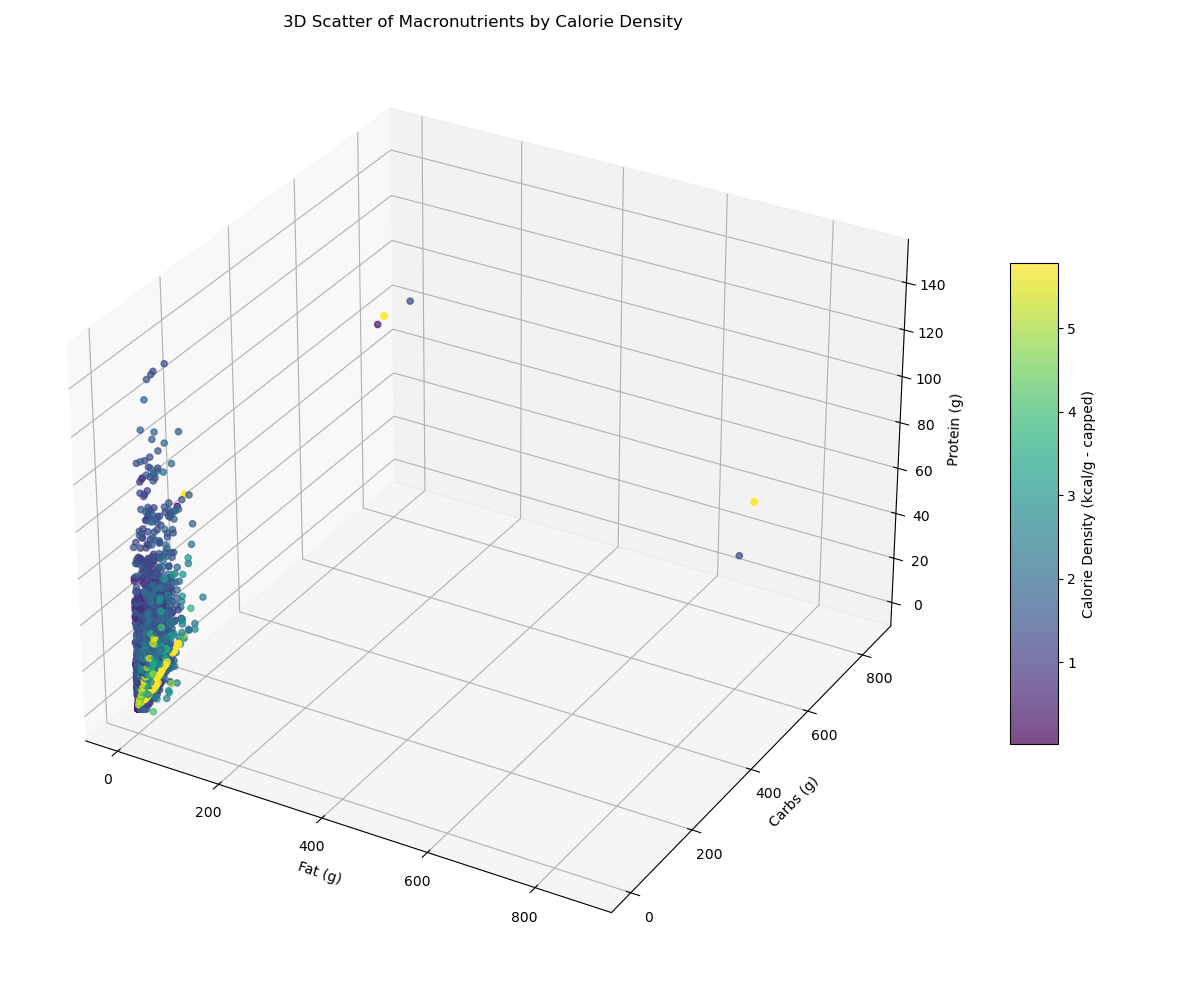
\includegraphics[width=\textwidth]{data/2.2clean/preoutlier.png}
                \caption{Macronutrient distribution before outlier removal. Note the stretched axes due to the extreme points.}
                \label{fig:macros_raw}
            \end{subfigure}
            \hfill
            \begin{subfigure}[b]{0.49\textwidth}
                \centering
                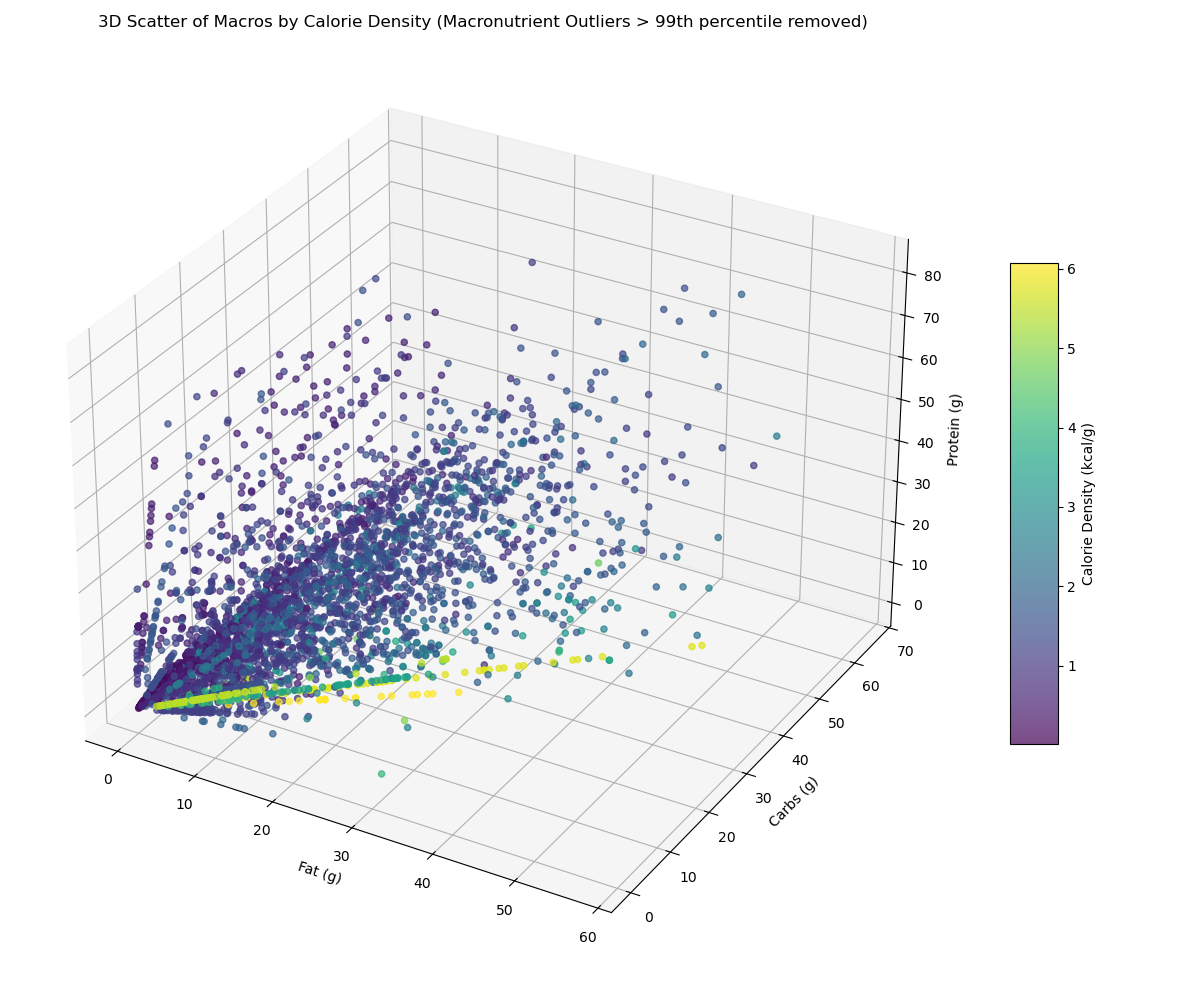
\includegraphics[width=\textwidth]{data/2.2clean/postoutlier.png}
                \caption{Macronutrient distribution after per-100 g percentile capping and plausibility cleaning.}\label{fig:macros_cleaned}
            \end{subfigure}
            \caption{3D scatter plot of macronutrients (fat, carbs, protein) colored by calorie density, shown before and after cleaning. The data cleaning process makes the central cluster of common dishes items more apparent.}\label{fig:macro_cleaning_3d}
            \end{figure}

        As a final sanity check, we compute the Pearson correlation matrix for the five target variables to assess dataset nutritional consistency. See Figure~\ref{fig:correlation_heatmap}.

        \begin{figure}[ht]
            \centering
            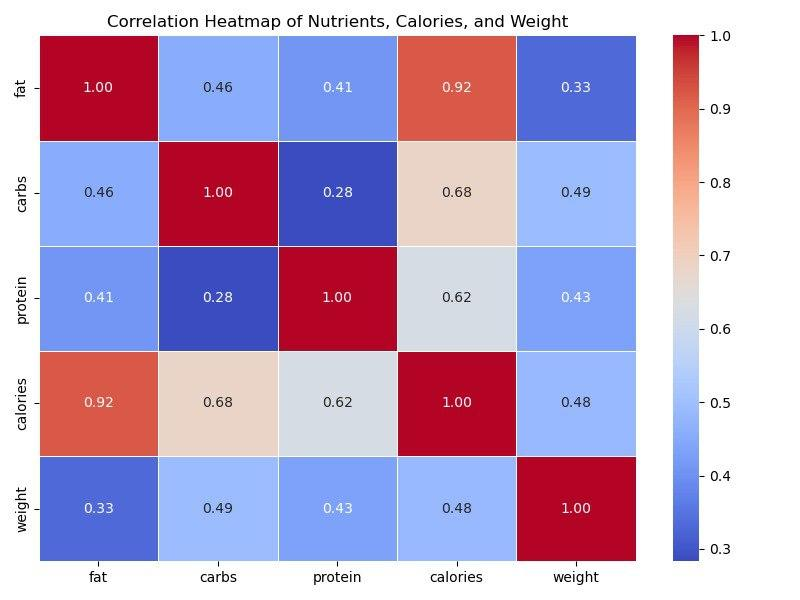
\includegraphics[width=0.7\textwidth]{data/2.2clean/heatmap.jpg}
            \caption{Correlation heatmap of the target nutritional variables after data cleaning.}\label{fig:correlation_heatmap}
        \end{figure}
        
        Fat demonstrates the highest correlation with calories (0.92), significantly higher than carbohydrates (0.68) and protein (0.62), which aligns with their respective energy densities, while dish weight shows expected moderate positive correlation.
        
        Thus, the cleaned dataset is a reliable foundation for training a multi-target nutritional prediction model.

        \clearpage
        
        \subsection{Data Augmentation via Frame Extraction}
        \label{subsec:frame_extraction}
        To improve model generalization, we decided to take advantage of videos by  extracting frames from them and using them as distinct data entries. However, if we take every frame for our dataset we will end up with terabytes of data which is unmanageable within our capacities. 
        Therefore, we need to understand how to extract small enough amount of frames to preserve lightning variability and viewpoint diversity. 
        
        One way to distinguish them is performing Principal Component Analysis (PCA) and select frames from different clusters. We utilize the Gaussian Mixture Model (GMM) to find the best clustering. As a criterion we test for $k$ = 1...10 clusters to predict and calculate the Bayesian Information Criterion (BIC).
         BIC would give us the best number of clusters that we should pick per video. 
        \begin{figure}[hbt!]
            \centering
            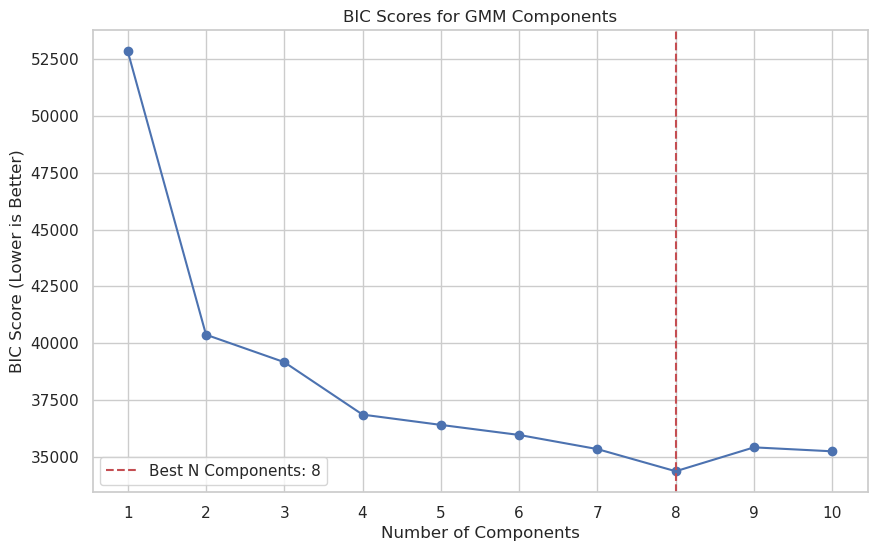
\includegraphics[width=0.7\linewidth]{data/Elbow rule.png}
            \caption{BIC Scores for different clusters $1..10$. \textit{It is important to say, that trying to fit for more clusters (more than 10) may get better results, but we don't have the capacity either way to take so many frames in the first place.}}
        \end{figure}
        The best BIC score is achieved for 8 clusters per video. However, taking 8 frames per video would result in approximately 160 GB of training data, which is not feasible considering our limitations. Therefore, using the elbow rule we can safely take 2 frames, which expand our dataset by 8 times. Even though the frames form clusters that are not necessarily independent, they are still sufficiently diverse to be considered as training data entries. 
        \begin{figure}[hbt!]
          \centering
          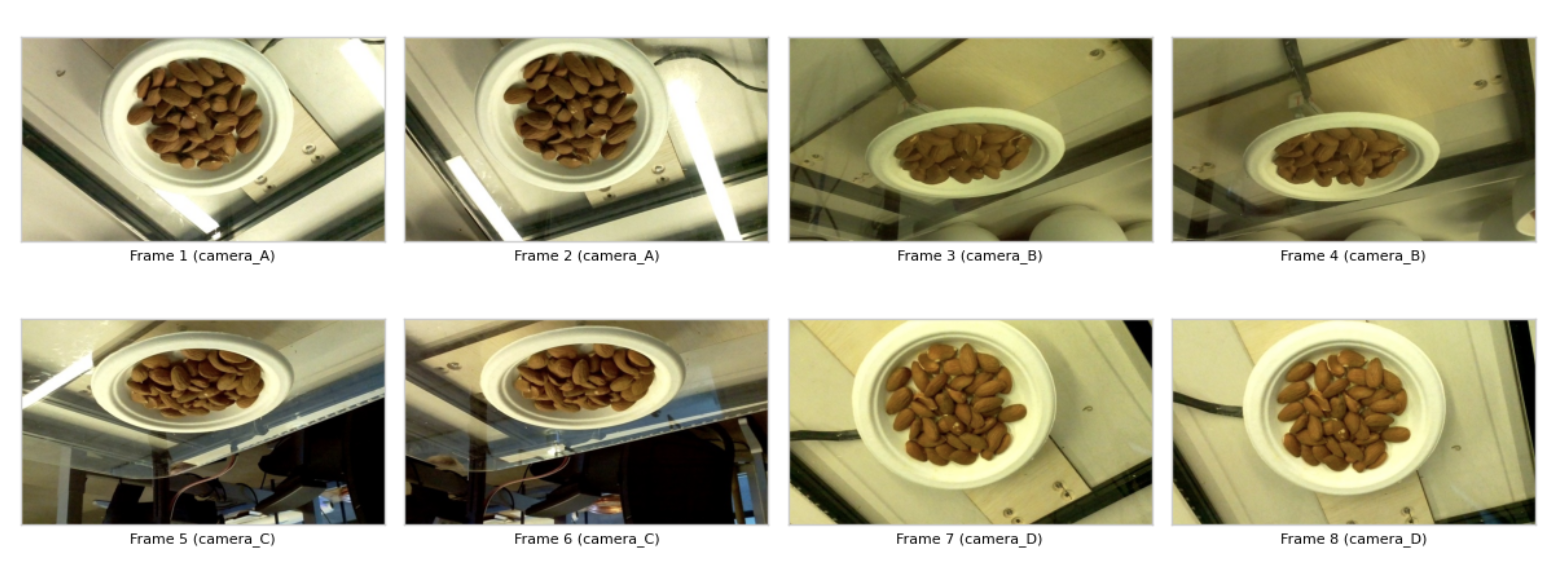
\includegraphics[width=1\textwidth]{data/8frames.png}
          \caption*{(a) Extracted frames from one dish video}
        
          \vspace{1em}
        
          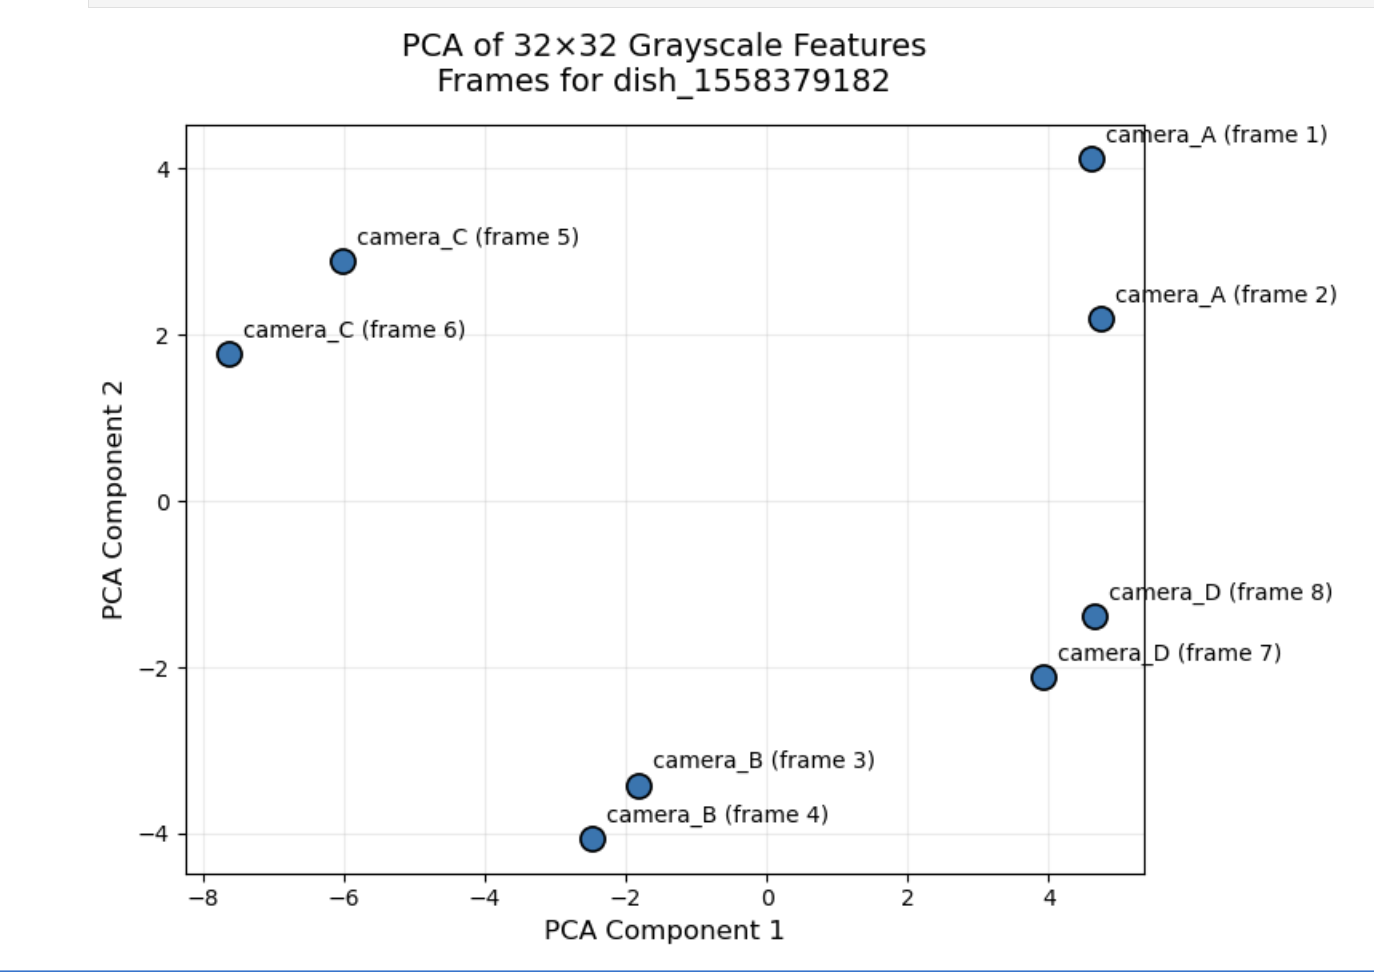
\includegraphics[width=0.6\textwidth]{data/2frames.png}
          \caption*{(b) PCA of grayscale frame embeddings}
        
          \caption{Examples of extracted frames and their PCA projection. Frame diversity captures changes in viewpoint and lighting, forming distinct visual clusters.}
          \label{fig:frame_extraction}
        \end{figure}

        The example in Figure~\ref{fig:frame_extraction} illustrates how the process works for a single dish. We can see that the extracted frames, when projected using PCA, form 4 visually distinct clusters corresponding to different camera angles. Although each cluster contains 2 images, it is not a problem, since we are applying the same rule uniformly across all dishes. Moreover, this allows to capture viewpoint and lighting variability. Therefore, our data augmentation approach is consistent, and it is used throughout the remainder of the pipeline.


        \clearpage
        
        \section{Segmentation Analysis}
        \subsection{Motivation and Problem Formulation}
        
            During early testing, our CNN regressors exhibited instability when trained on raw images with cluttered backgrounds and variable lighting. Small portions occupying a tiny fraction of the plate were particularly problematic. This motivated us to investigate the addition of a segmentation preprocessing stage.
            
            The following failure modes were identified after visual inspection of predictions on similar dishes, where the only main differences were the additional presence of items in the background (1) and/or shadow artifacts (2):
            \begin{enumerate}
                \item Models seem to incorporate non-food elements including plates and utensils into nutritional predictions, leading to systematic overestimation.
                \item Lighting variations and shadows caused inconsistent predictions for identical food items, often leading to underestimation.
            \end{enumerate}
        
            \begin{figure}[h!]\label{fig:seg_highest_pred_err_examples}
                \centering
                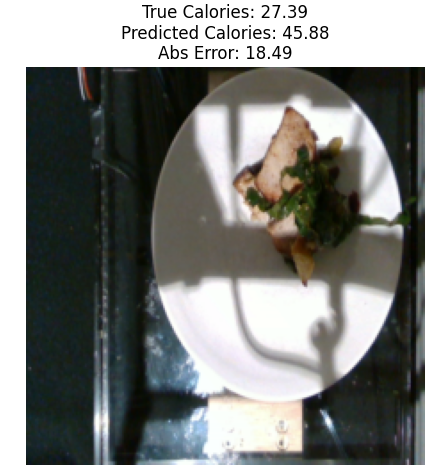
\includegraphics[width=0.21\linewidth]{data/2.3seg/seg_highest_pred_err_examples_2.png}
                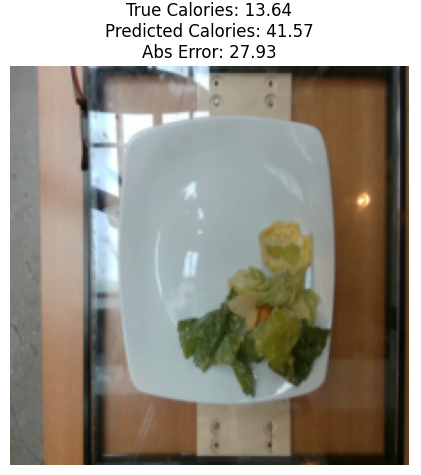
\includegraphics[width=0.20\linewidth]{data/2.3seg/seg_highest_pred_err_examples_3.png}
                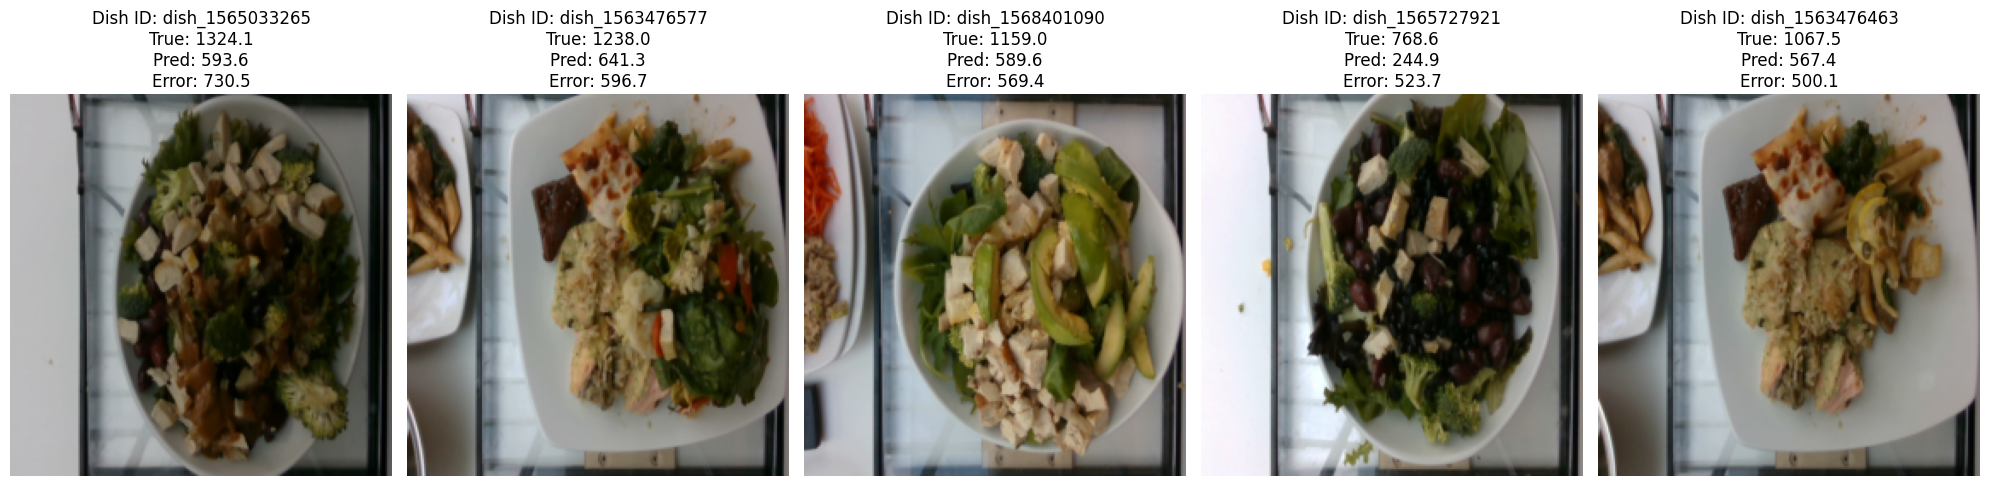
\includegraphics[width=0.9\linewidth]{data/2.3seg/seg_highest_pred_err_examples.png}
                \caption{Examples of failure cases that led to this segmentation experiment.}
            \end{figure}
            
            To address these challenges, we experiment with a segmentation preprocessing stage, with the goal of focusing the model on nutritionally relevant regions. This is done during both training and inference to evaluate the impact of this preprocessing according to the metrics defined in \autoref{sec:metrics}.
        
        \clearpage

        \subsection{U²-Net}
        After testing different YOLO \cite{redmon2016yolo} models, as well as SAM \cite{kirillov2023sam} models, we chose U$^2$-Net~\cite{qin2020u2net} as our primary segmentation backbone as it demonstrates good performance in salient object detection. Most importantly, the nested U$^2$-Net architecture is capable of extracting features at multiple scales, which is essential as dishes often present diverse textures/colors/ingredients that require different levels of abstraction for accurate segmentation.
        
        \subsection{Implementation and Training Details}
        Nutrition5K does not include ground-truth segmentation masks. Since our goal is not to train a segmentation model, we adopt a saliency-based strategy centered on a publicly available U$^2$-Net checkpoint~\cite{qin2020u2net} trained for general salient object detection. We decide not to fine-tune nor train from scratch on food segmentation datasets because of the time and computational constraints of the project.
        
        \paragraph{Input preprocessing}
        We adopt a 64/16/20 train/val/test split. Images are resized to $224\times224$ and normalized using ImageNet statistics (mean $[0.485, 0.456, 0.406]$, std $[0.229, 0.224, 0.225]$) to match the expected output from the used U$^2$-Net checkpoint. We apply simple augmentations (random horizontal flips, random rotations and small color jitter) to encourage robustness to illumination changes as well as generalization to different viewpoints.

        \paragraph{Loss function}
        Segmentation being used purely as a preprocessing stage, the regression CNN is trained with mean squared error (MSE) on the target variables:
        \begin{align}
            \hat{y}_i &= f_{\theta}(x_i) \in \mathbb{R}^D, \quad y_i \in \mathbb{R}^D, \\
            \mathcal{L}_{\mathrm{MSE}} &= \frac{1}{ND} \sum_{i=1}^{N} \sum_{d=1}^{D} \big{(\hat{y}_{i,d} - y_{i,d}\big)}^2.
        \end{align}
        where $x_i$ denotes the preprocessed RGB image fed to the regressor (either raw or segmented; tensor of shape $3\times224\times224$), $f_{\theta}$ is the ResNet50-based regression network with learnable parameters $\theta$, $\hat{y}_i\in\mathbb{R}^D$ is the predicted vector (e.g., calories only $D{=}1$; calories+weight $D{=}2$; all targets such as calories+protein+carbs+fat $D{=}4$), $y_i\in\mathbb{R}^D$ is the ground-truth vector, $D$ is the number of target variables, $i$ indexes samples in a mini-batch, and $N$ is the number of samples in the current mini-batch.
        
        \paragraph{Optimization and regularization}
        We use AdamW (initial learning rate $1\times10^{-3}$, weight decay $1\times10^{-4}$) together with ReduceLROnPlateau on the validation loss (factor $0.2$, patience equal to half of the early-stopping patience; $5$). Early stopping monitors validation loss with patience $10$, and the best model checkpoint is saved whenever the monitored loss improves.

        \subsection{Segmentation Pipeline and Evaluation Methodology}
        The complete segmentation pipeline takes raw food images and outputs isolated food regions (background is composited to black) through the following process:
        
        For any given dish image, the pipeline checks if a segmentation mask has already been computed and cached, in which case it uses it. Otherwise, the U$^2$-Net model is used to compute a grayscale saliency map which is then thresholded at $\tau{=}0.5$ into a binary mask. The latter is applied to the original image to highlight the main food items.
        The resulting image is then cropped to an axis-aligned bounding box of the largest contour (largest connected component, supposed to be the food region on the dish).
        
        \paragraph{Architectures evaluated in segmentation experiments}
        We paired the preprocessing conditions with the following ResNet50-based regressor:
        \begin{itemize}
            \item \textbf{ResNet50-based regressor:} ResNet50 backbone (frozen) with an MLP head.
        \end{itemize}
        
        \begin{figure}[h]
        \centering
        \resizebox{\textwidth}{!}{
        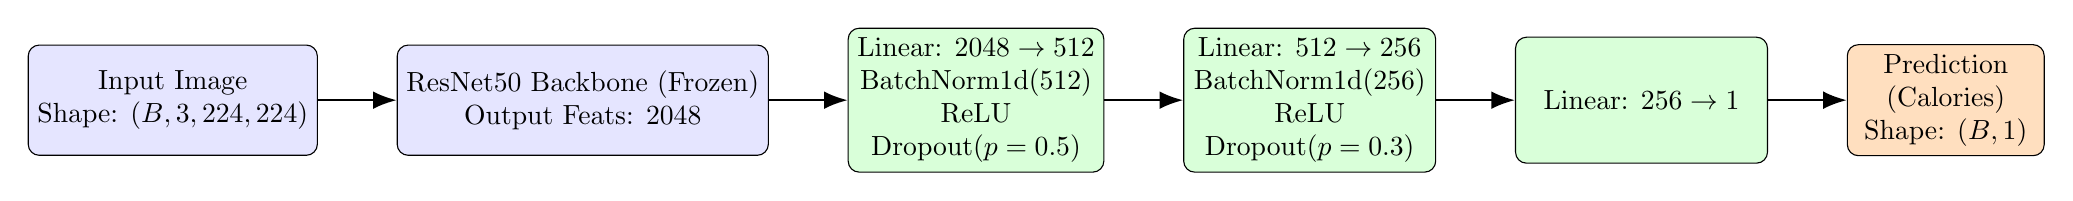
\begin{tikzpicture}[node distance=1.5cm and 1cm]
        % Input
        \node[block] (input) {Input Image \\ Shape: $(B, 3, 224, 224)$};
        
        % Backbone
        \node[block, right=of input] (backbone) {ResNet50 Backbone (Frozen) \\ Output Feats: $2048$};
        
        % FC1
        \node[head, right=of backbone] (fc1) {Linear: $2048 \rightarrow 512$ \\ BatchNorm1d(512) \\ ReLU \\ Dropout($p=0.5$)};
        
        % FC2
        \node[head, right=of fc1] (fc2) {Linear: $512 \rightarrow 256$ \\ BatchNorm1d(256) \\ ReLU \\ Dropout($p=0.3$)};
        
        % Output layer
        \node[head, right=of fc2] (fc3) {Linear: $256 \rightarrow 1$};
        
        % Output
        \node[output, right=of fc3] (output) {Prediction \\ (Calories) \\ Shape: $(B, 1)$};
        
        % Connections
        \draw[arrow] (input) -- (backbone);
        \draw[arrow] (backbone) -- (fc1);
        \draw[arrow] (fc1) -- (fc2);
        \draw[arrow] (fc2) -- (fc3);
        \draw[arrow] (fc3) -- (output);
        \end{tikzpicture}
        }
        \caption{ResNet50-based regressor. 
        \textbf{Total parameters:} $\sim 24.6$M (\textit{frozen backbone:} $\sim 23.5$M), 
        \textbf{trainable parameters:} $\sim 1.18$M}
        \label{fig:resnet50_complex}
        \end{figure}
        
        
        \subsubsection{Experimental Setup}
        To quantify the impact of this segmentation pipeline and to assess its relevance as a preprocessing step, we conducted controlled experiments and compared three image preprocessing approaches in total:
        \begin{enumerate}
            \item Original RGB images without preprocessing
            \item Simple geometric square cropping based at the center of the images
            \item Full segmentation pipeline with blacked-out background as described above.
        \end{enumerate}
                
        
        \subsubsection{Testing protocol}
            To isolate the effect of the segmentation preprocessing, we hold relevant RNG seeds, the regressor head architecture, optimizer hyperparameters, and training schedule fixed across all tests.
            
            We defined a protocol to assess the performance impact of segmentation vs.\ no segmentation.
            The following configurations were evaluated:
        
            \begin{table}[h!]
                \centering
                \caption{Segmentation testing protocol matrix}
                \label{tab:seg_test_protocol}
                \resizebox{\textwidth}{!}{
                \begin{tabular}{|l|l|l|l|}
                \hline
                \textbf{Model} & \textbf{Target} & \textbf{Dataset} & \textbf{Segmentation} \\ \hline
                ResNet50 regressor & Calories & Overhead only & No / Yes \\ \hline
                ResNet50 regressor & Calories & Overhead + Extracted (PCA+GMM) & No / Yes \\ \hline
                ResNet50 regressor & All nutrients & Overhead only & No / Yes \\ \hline
                \end{tabular}
                }
            \end{table}
            
        \subsection{Results and Discussion}
        Contrary to our initial expectations, the segmentation preprocessing step does not improve nutritional prediction accuracy. Possible suspects include the loss of information (contextual cues such as plate scale) and undesired artifacts from the segmentation process on some challenging samples, as can be seen in \autoref{fig:segmentation_examples}. 
        
        We also conduct a qualitative analysis of some predictions with the segmentation step through visual inspection. The pre-trained U$^2$-Net segmentation model performs particularly well on dishes with high contrast between food and background, instances in which the segmentation masks successfully exclude unrelated elements from the image such as cutlery or tableware. We however also observe both over-segmentation of dissimilar food items (e.g., separating sauce from base ingredients) and segmentation failures on some challenging samples (e.g., food lies in the blacked-out area).
        
        \begin{figure}[h!]
            \centering
            % Successful segmentation cases
            \begin{subfigure}[b]{0.48\textwidth}
                \centering
                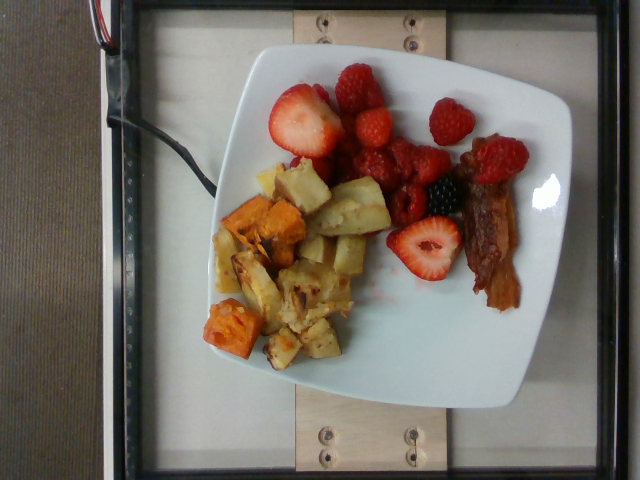
\includegraphics[width=0.3\textwidth]{data/2.3seg/1.png}
                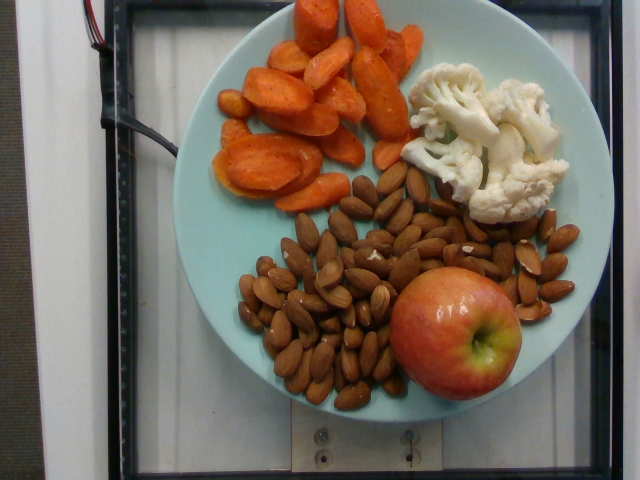
\includegraphics[width=0.3\textwidth]{data/2.3seg/2.png}
                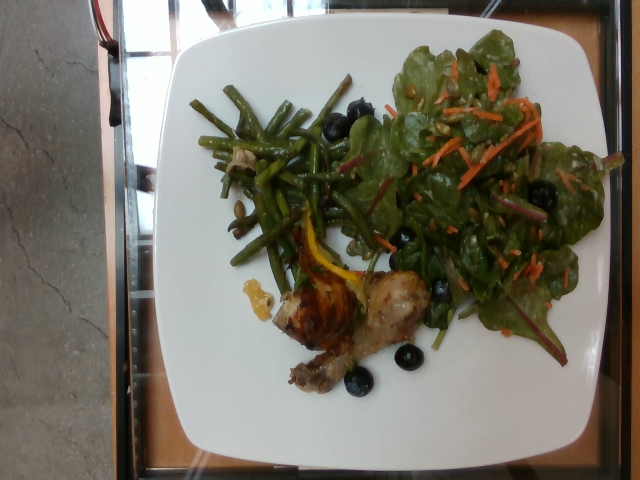
\includegraphics[width=0.3\textwidth]{data/2.3seg/3.png}
                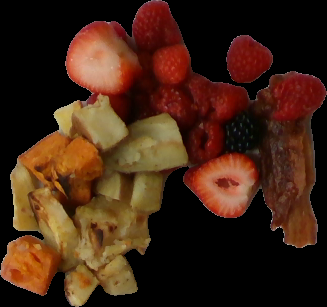
\includegraphics[width=0.3\textwidth]{data/2.3seg/1s.png}
                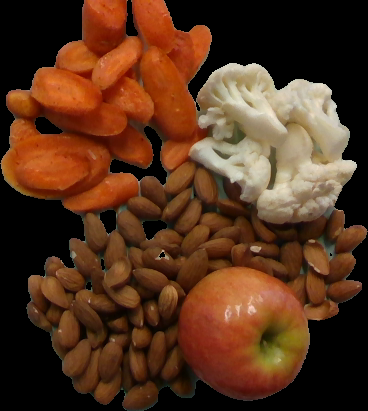
\includegraphics[width=0.3\textwidth]{data/2.3seg/2s.png}
                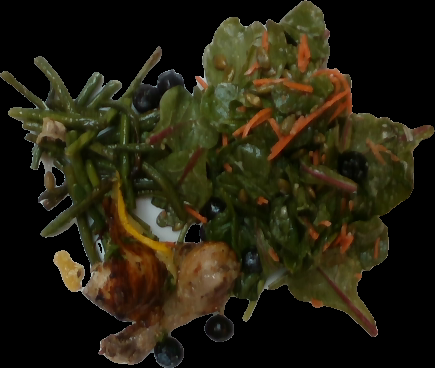
\includegraphics[width=0.3\textwidth]{data/2.3seg/3s.png}
                \caption{Successful segmentation cases}
                \label{fig:seg_success}
            \end{subfigure}
            \hfill
            % Failure segmentation cases
            \begin{subfigure}[b]{0.48\textwidth}
                \centering
                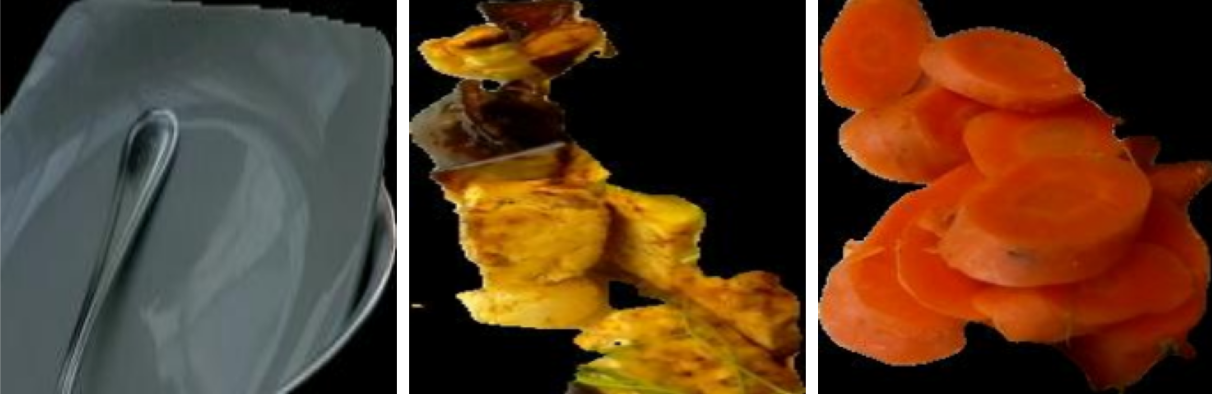
\includegraphics[width=0.9\textwidth]{data/2.3seg/seg_failures_1.png}
                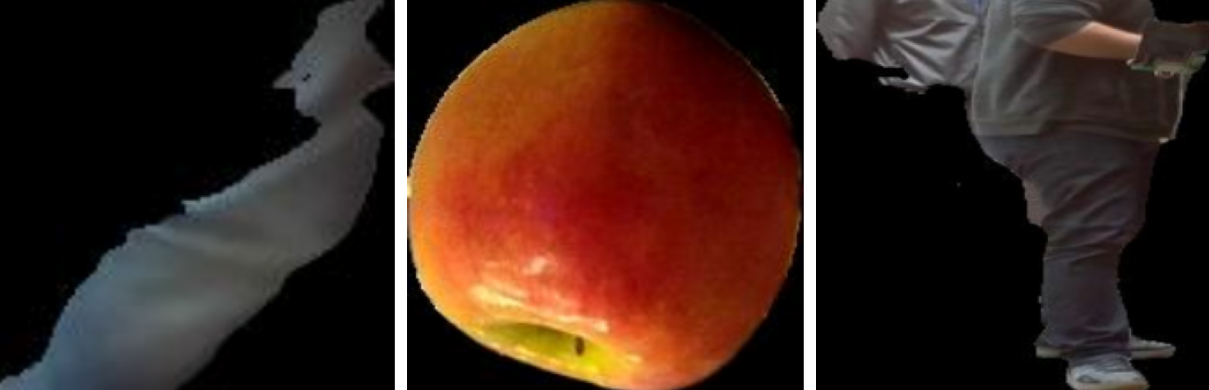
\includegraphics[width=0.9\textwidth]{data/2.3seg/seg_failures_2.png}
                \caption{Challenging segmentation cases}
                \label{fig:seg_failure}
            \end{subfigure}
            \caption{U²-Net segmentation performance across different food types}
            \label{fig:segmentation_examples}
        \end{figure}
        


        % big boi r&g comparative table
        \begin{table}[H]
            \centering
            \caption{Comparative Prediction Performance: Without vs. With Segmentation}
            \label{tab:comparison}
            
            % --- Step 1: Save the entire tabular environment into the savebox ---
            % This measures the table's dimensions but doesn't display it yet.
            \begin{lrbox}{\mycomparisonboxtable}
            \begin{tabular}{@{}llcccc@{}}
            \toprule
            \textbf{Nutrient} & \textbf{Metric} & \textbf{Without Seg.} & \textbf{With Seg.} & \textbf{Change (\%)} \\
            \midrule
            % --- Calories ---
            \multirow{4}{*}{\textbf{Calories}} 
            & MAE       & \textbf{81.27}  & 90.36  & \textcolor{badred}{+11.18\% $\uparrow$} \\
            & MAE (\%)  & \textbf{31.91}  & 35.48  & \textcolor{badred}{+11.18\% $\uparrow$} \\
            & RMSE      & \textbf{116.98} & 130.89 & \textcolor{badred}{+11.89\% $\uparrow$} \\
            & R²        & \textbf{0.68}   & 0.60   & \textcolor{badred}{-11.76\% $\downarrow$} \\
            \addlinespace % Adds a little space between nutrient groups
            % --- Weight ---
            \multirow{4}{*}{\textbf{Weight}}   
            & MAE       & \textbf{46.09}  & 64.87  & \textcolor{badred}{+40.75\% $\uparrow$} \\
            & MAE (\%)  & \textbf{20.79}  & 29.27  & \textcolor{badred}{+40.79\% $\uparrow$} \\
            & RMSE      & \textbf{65.05}  & 89.59  & \textcolor{badred}{+37.72\% $\uparrow$} \\
            & R²        & \textbf{0.82}   & 0.66   & \textcolor{badred}{-19.51\% $\downarrow$} \\
            \addlinespace
            % --- Fat ---
            \multirow{4}{*}{\textbf{Fat}}      
            & MAE       & 7.25   & \textbf{6.45}   & \textcolor{goodgreen}{-11.03\% $\downarrow$} \\
            & MAE (\%)  & 58.20  & \textbf{51.81}  & \textcolor{goodgreen}{-10.98\% $\downarrow$} \\
            & RMSE      & 10.27  & \textbf{9.95}   & \textcolor{goodgreen}{-3.12\% $\downarrow$} \\
            & R²        & 0.43   & \textbf{0.46}   & \textcolor{goodgreen}{+6.98\% $\uparrow$} \\
            \addlinespace
            % --- Carbs ---
            \multirow{4}{*}{\textbf{Carbs}}    
            & MAE       & \textbf{9.54}   & 10.44  & \textcolor{badred}{+9.43\% $\uparrow$} \\
            & MAE (\%)  & \textbf{49.40}  & 54.04  & \textcolor{badred}{+9.40\% $\uparrow$} \\
            & RMSE      & \textbf{12.98}  & 14.05  & \textcolor{badred}{+8.24\% $\uparrow$} \\
            & R²        & \textbf{0.34}   & 0.23   & \textcolor{badred}{-32.35\% $\downarrow$} \\
            \addlinespace
            % --- Protein ---
            \multirow{4}{*}{\textbf{Protein}}  
            & MAE       & \textbf{9.59}   & 10.12  & \textcolor{badred}{+5.53\% $\uparrow$} \\
            & MAE (\%)  & \textbf{50.77}  & 53.54  & \textcolor{badred}{+5.46\% $\uparrow$} \\
            & RMSE      & \textbf{14.22}  & 15.29  & \textcolor{badred}{+7.52\% $\uparrow$} \\
            & R²        & \textbf{0.55}   & 0.48   & \textcolor{badred}{-12.73\% $\downarrow$} \\
            \bottomrule
            \end{tabular}
            \end{lrbox}
            % --- Step 2: Display the saved table and the note below it ---
            \usebox{\mycomparisonboxtable} % This displays the table
            \vspace{1ex} % Add a small vertical space
            % Create a minipage with the *exact width* of the table (\wd\mycomparisonboxtable)
            \begin{minipage}{\wd\mycomparisonboxtable}
            \small\emph{Note: \textbf{Bold} values indicate the best performance. 
            The ``Change (\%)'' column shows the performance shift from the ``Without Seg'' model to the ``With Seg'' model. 
            \textcolor{goodgreen}{Green indicates an improvement} (lower error, higher $R^2$), 
            while \textcolor{badred}{red indicates a decline}.}
            \end{minipage}
        \end{table}
        
        % \begin{figure}[h!]
        % \centering
        % \begin{minipage}[t]{\textwidth}
        %     \centering
        %     \captionof{table}{Prediction Performance - without segmentation}
        %     \label{tab:without_segmentation}
        %     \begin{tabular}{@{}lcccccc@{}}
        %     \toprule
        %     \textbf{Nutrient} & \textbf{MAE} & \textbf{MAE (\%)} & \textbf{RMSE} & \textbf{R²} & \textbf{Mean True} & \textbf{Mean Pred} \\
        %     \midrule
        %     Calories & \textbf{81.27}  & \textbf{31.91} & \textbf{116.98} & \textbf{0.68} & 254.71 & 250.89 \\
        %     Weight   & \textbf{46.09}  & \textbf{20.79} & \textbf{65.05}  & \textbf{0.82} & 221.65 & 208.10 \\
        %     Fat      & 7.25   & 58.20 & 10.27  & 0.43 & 12.45  & 15.11  \\
        %     Carbs    & \textbf{9.54}   & \textbf{49.40} & \textbf{12.98}  & \textbf{0.34} & 19.31  & 17.99  \\
        %     Protein  & \textbf{9.59}   & \textbf{50.77} & \textbf{14.22}  & \textbf{0.55} & 18.90  & 20.37  \\
        %     \bottomrule
        %     \end{tabular}
        % \end{minipage}
        % \end{figure}
        
        % \begin{figure}[h!]
        % \centering
        % \begin{minipage}[t]{\textwidth}
        %     \centering
        %     \captionof{table}{Prediction Performance - with segmentation}
        %     \label{tab:with_segmentation}
        %     \begin{tabular}{@{}lcccccc@{}}
        %     \toprule
        %     \textbf{Nutrient} & \textbf{MAE} & \textbf{MAE (\%)} & \textbf{RMSE} & \textbf{R²} & \textbf{Mean True} & \textbf{Mean Pred} \\
        %     \midrule
        %     Calories & 90.36  & 35.48 & 130.89 & 0.60 & 254.71 & 247.79 \\
        %     Weight   & 64.87  & 29.27 & 89.59  & 0.66 & 221.65 & 213.92 \\
        %     Fat      & \textbf{6.45}   & \textbf{51.81} & \textbf{9.95}   & \textbf{0.46} & 12.45  & 12.29  \\
        %     Carbs    & 10.44  & 54.04 & 14.05  & 0.23 & 19.31  & 18.49  \\
        %     Protein  & 10.12  & 53.54 & 15.29  & 0.48 & 18.90  & 18.63  \\
        %     \bottomrule
        %     \end{tabular}
        % \end{minipage}
        % \end{figure}
                
        \subsubsection{Impact on Final Architecture}
        Given the observed performance degradations (except a small improvement for fat), we remove segmentation in the final model and retain the simpler center cropping step that preserves contextual cues and reduces compute.
        
        
        
        
        
        \clearpage
                
        \section{Dish Weight Estimation}
        This part of the project focuses on specifically estimating the total weight of a dish from a single image. We took this approach because we believe that accurate weight estimation is fundamental in determining all the nutritional components. On top of that, it allows the conversion of relative nutrition estimations (from our \%-estimation models) into numerical values, which we do later in the pipeline. 
        
        We explore two different model architectures (built from scratch) of increasing complexity and test them on both the original Nutrition 5K dataset and the augmented one (see \autoref{subsec:frame_extraction}). Our results demonstrate that deeper architectures combined with the augmented dataset lead to better performance, achieving a relative MAE of 18.68\% on the testing dataset.

        \subsection{Model Architectures}
        We design and implement two CNN architectures with varying complexity to understand the relationship between model capacity and weight estimation performance. \\

        \begin{figure}[h]
        \centering
        \resizebox{\textwidth}{!}{
        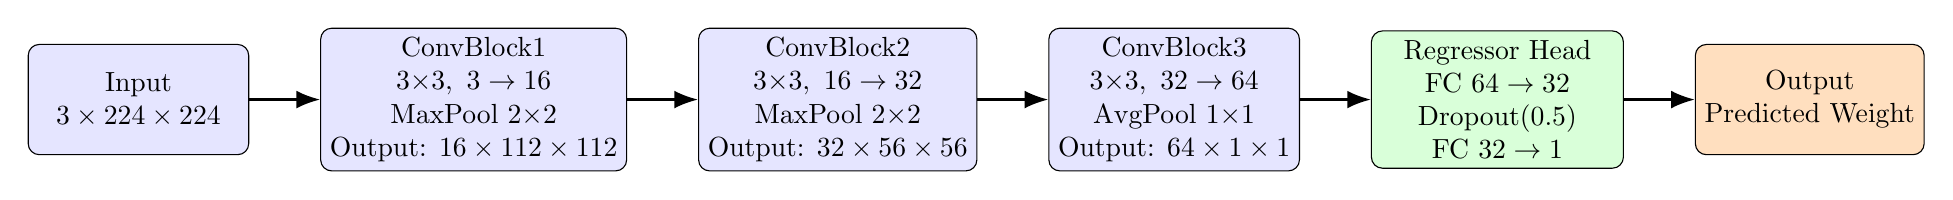
\begin{tikzpicture}[node distance=1.5cm and 0.9cm]
          \node[block] (input) {Input \\ $3 \times 224 \times 224$};
        
          \node[block, right=of input] (conv1) {ConvBlock1 \\ $3{\times}3,\ 3 \rightarrow 16$ \\ MaxPool $2{\times}2$ \\ Output: $16 \times 112 \times 112$};
        
          \node[block, right=of conv1] (conv2) {ConvBlock2 \\ $3{\times}3,\ 16 \rightarrow 32$ \\ MaxPool $2{\times}2$ \\ Output: $32 \times 56 \times 56$};
        
          \node[block, right=of conv2] (conv3) {ConvBlock3 \\ $3{\times}3,\ 32 \rightarrow 64$ \\ AvgPool $1{\times}1$ \\ Output: $64 \times 1 \times 1$};
        
          \node[head, right=of conv3] (head) {Regressor Head \\ FC $64 \rightarrow 32$ \\ Dropout(0.5) \\ FC $32 \rightarrow 1$};
        
          \node[output, right=of head] (output) {Output \\ Predicted Weight};
        
          \draw[arrow] (input) -- (conv1);
          \draw[arrow] (conv1) -- (conv2);
          \draw[arrow] (conv2) -- (conv3);
          \draw[arrow] (conv3) -- (head);
          \draw[arrow] (head) -- (output);
        \end{tikzpicture}
        }
        \caption{SimpleCNN architecture for weight estimation (25k parameters)}
        \label{fig:simplecnn}
        \end{figure}
        
        \begin{figure}[h]
        \centering
        \resizebox{\textwidth}{!}{
        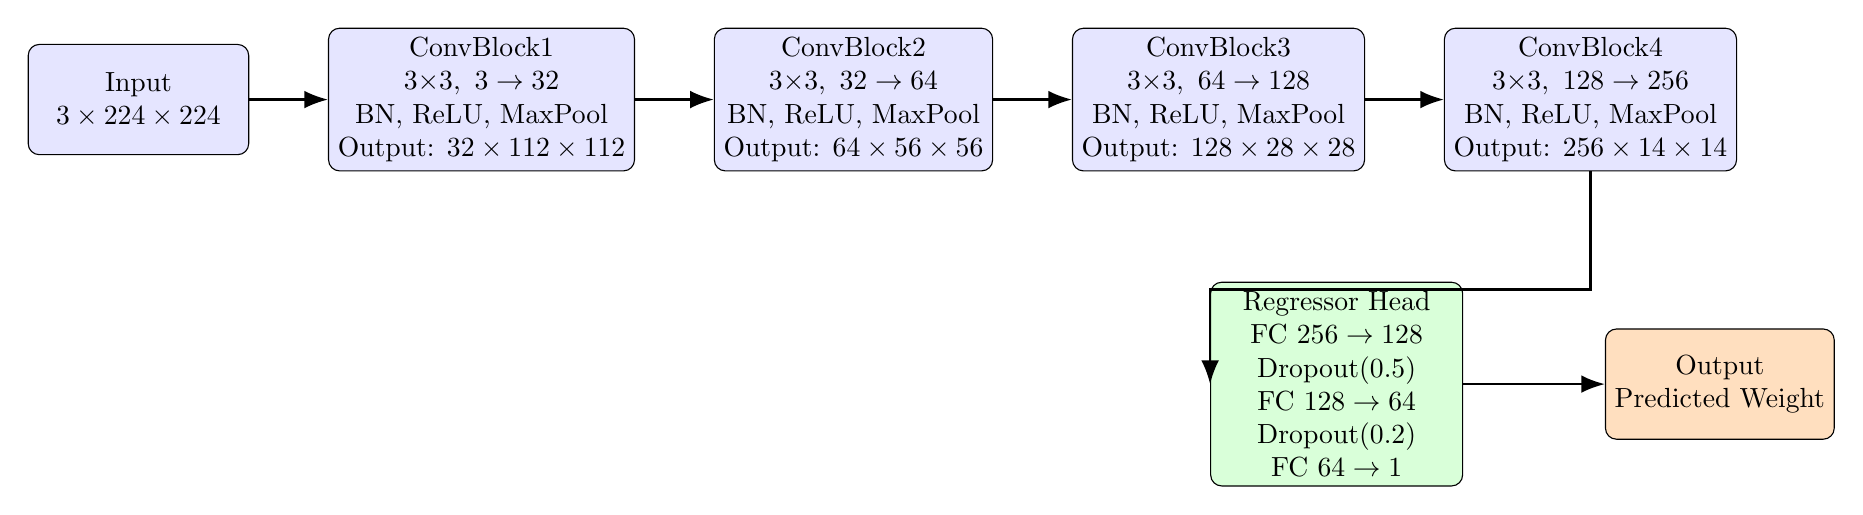
\begin{tikzpicture}[node distance=1.5cm and 1cm]
          \node[block] (input) {Input \\ $3 \times 224 \times 224$};
        
          \node[block, right=of input] (conv1) {ConvBlock1 \\ $3{\times}3,\ 3 \rightarrow 32$ \\ BN, ReLU, MaxPool \\ Output: $32 \times 112 \times 112$};
        
          \node[block, right=of conv1] (conv2) {ConvBlock2 \\ $3{\times}3,\ 32 \rightarrow 64$ \\ BN, ReLU, MaxPool \\ Output: $64 \times 56 \times 56$};
        
          \node[block, right=of conv2] (conv3) {ConvBlock3 \\ $3{\times}3,\ 64 \rightarrow 128$ \\ BN, ReLU, MaxPool \\ Output: $128 \times 28 \times 28$};
        
          \node[block, right=of conv3] (conv4) {ConvBlock4 \\ $3{\times}3,\ 128 \rightarrow 256$ \\ BN, ReLU, MaxPool \\ Output: $256 \times 14 \times 14$};
        
          \node[head, below=1.4cm of conv3, xshift=1.5cm] (head) {Regressor Head \\ FC $256 \rightarrow 128$ \\ Dropout(0.5) \\ FC $128 \rightarrow 64$ \\ Dropout(0.2) \\ FC $64 \rightarrow 1$};
        
          \node[output, right=1.8cm of head] (output) {Output \\ Predicted Weight};
        
          \draw[arrow] (input) -- (conv1);
          \draw[arrow] (conv1) -- (conv2);
          \draw[arrow] (conv2) -- (conv3);
          \draw[arrow] (conv3) -- (conv4);
          \draw[arrow] (conv4.south) -- ++(0,-1.5) -| (head.west);
          \draw[arrow] (head) -- (output);
        \end{tikzpicture}
        }
        
        \caption{DeepCNN architecture for weight estimation (430k parameters)}
        \label{fig:deepcnn}
        \end{figure}

        % SimpleCNN: a 3-block simple CNN with a 1-hidden-layer MLP head (25 k params)
        % \begin{figure}[h]
        %    \centering
        %    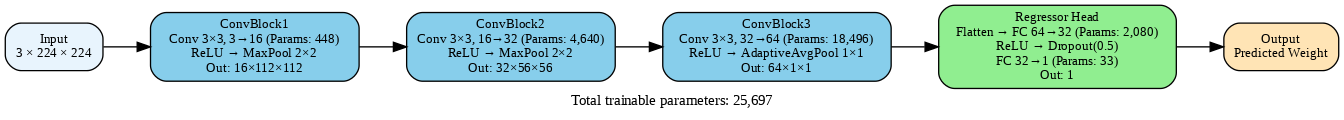
\includegraphics[width=1\textwidth]{data/simple_cnn_architecture.png}
        %    \caption{Simple CNN architecture for weight estimation}
        %    \label{fig:simple_cnn}
        % \end{figure} \\
        % DeepCNN: a 4-block Deep CNN with a hidden-layer MLP head (430 k params)
        % \begin{figure}[h]
        %    \centering
        %    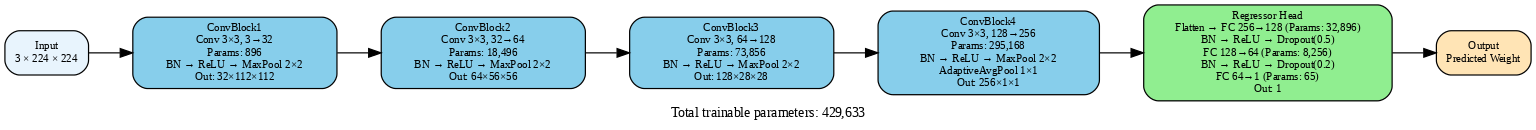
\includegraphics[width=1\textwidth]{data/deep_cnn_architecture.png}
        %    \caption{DeepCNN architecture for weight estimation}
        %    \label{fig:simple_cnn}
        % \end{figure}


        Additionally, we explore the benefit of data augmentation by training on an extended dataset where extra frames are extracted from side-angle dish videos. This augmentation increases data diversity in terms of lighting and viewpoint.

        
        
        \subsection{Performance Evaluation}

        The performance is assessed using the metrics fixed in the beginning. 
        \begin{table}[ht]
          \centering
          \caption{Dish‑weight prediction results on the Nutrition5K test split.
                   “Extended” denotes training with the two‑frame augmented set.}
          \label{tab:weight_results}
          \begin{tabular}{lrrrrrr}
            \toprule
            \textbf{Model} & \textbf{MAE} & \textbf{Rel.\ MAE (\%)} &
            \textbf{RMSE} & \textbf{R$^{2}$} &
            \textbf{Mean True} & \textbf{Mean Pred} \\
            \midrule
            Deep‑CNN (extended) & 43.89 & 18.68 & 63.12 & 0.82 & 234.9 & 229.2 \\
            Deep‑CNN            & 43.54 & 21.31 & 57.82 & 0.84 & 204.3 & 208.0 \\
            Simple‑CNN          & 76.11 & 37.26 & 103.91 & 0.49 & 204.3 & 202.3 \\
            \bottomrule
          \end{tabular}
        \end{table}

        \textbf{Baseline performance:} On the original Nutrion5K dataset, the DeepCNN model performed noticeably better than the SimpleCNN model, lowering the MAE by 43\% and raising R$^2$ from 0.49 to 0.84. At the same time, the relative MAE was improved significantly, going from 37.26\% to 21.31\%. These findings suggest that the more complex architecture more effectively captured the visual characteristics required for accurate weight estimation

       \textbf{ Impact of Data Augmentation:} Using the augmented dataset resulted in further performance improvement.  The R$^2$ remained roughly constant at 0.82, while the DeepCNN model generated a lower relative MAE, falling to 18.68\%. These results validated the data augmentation strategy and confirmed that combining the more complex architecture with the augmented dataset resulted in the best performance.

       Later in the pipeline, we proceeded with the DeepCNN model trained on the augmented dataset for the weight estimation part. 


        
        \section{Relative Nutrient Estimation (per 100g)}
        \subsection{Comparative Model Analysis}
        The approach we chose is different to predicting absolute values. We train two models separately - one predicting the weight of the food on the picture and another one predicting how many nutrition per 100g in this meal. This result for a picture is later multiplied by the weight predicted, to achieve the total nutrition per meal. We were inspired by the paper model with well-researched architecture and tried to enhance it to suit our limitations and resources. We compared the four categories of models.
        \begin{itemize}
        \item \textbf{Simple CNN:} Simple Convolutional Network to better understand the task and set a baseline fundamental performance.
        \item \textbf{DeepCNN:} A deeper custom architecture, designed to test the performance limits of a network trained from scratch.
        \item \textbf{MobileLikeNet:} A lightweight computationally efficient model designed for applied user-case of deployment on mobile phones.
        \item \textbf{ResNet34:} A deep, pre-trained model utilizing transfer learning, aiming for best performance.
    \end{itemize}
        - starting from SimpleCNN exploratory model for eased understanding of the problem to ResNet34 - heavy pre-trained model to achieve best theoretical results. 
        
        All models were trained with a batch size of 32 for 200 epochs, using 80\% of the data per epoch and an early stopping patience of 10.
 

%         \begin{figure}[h!]
%     \centering
%     \begin{subfigure}[b]{\textwidth}
%         \centering
%         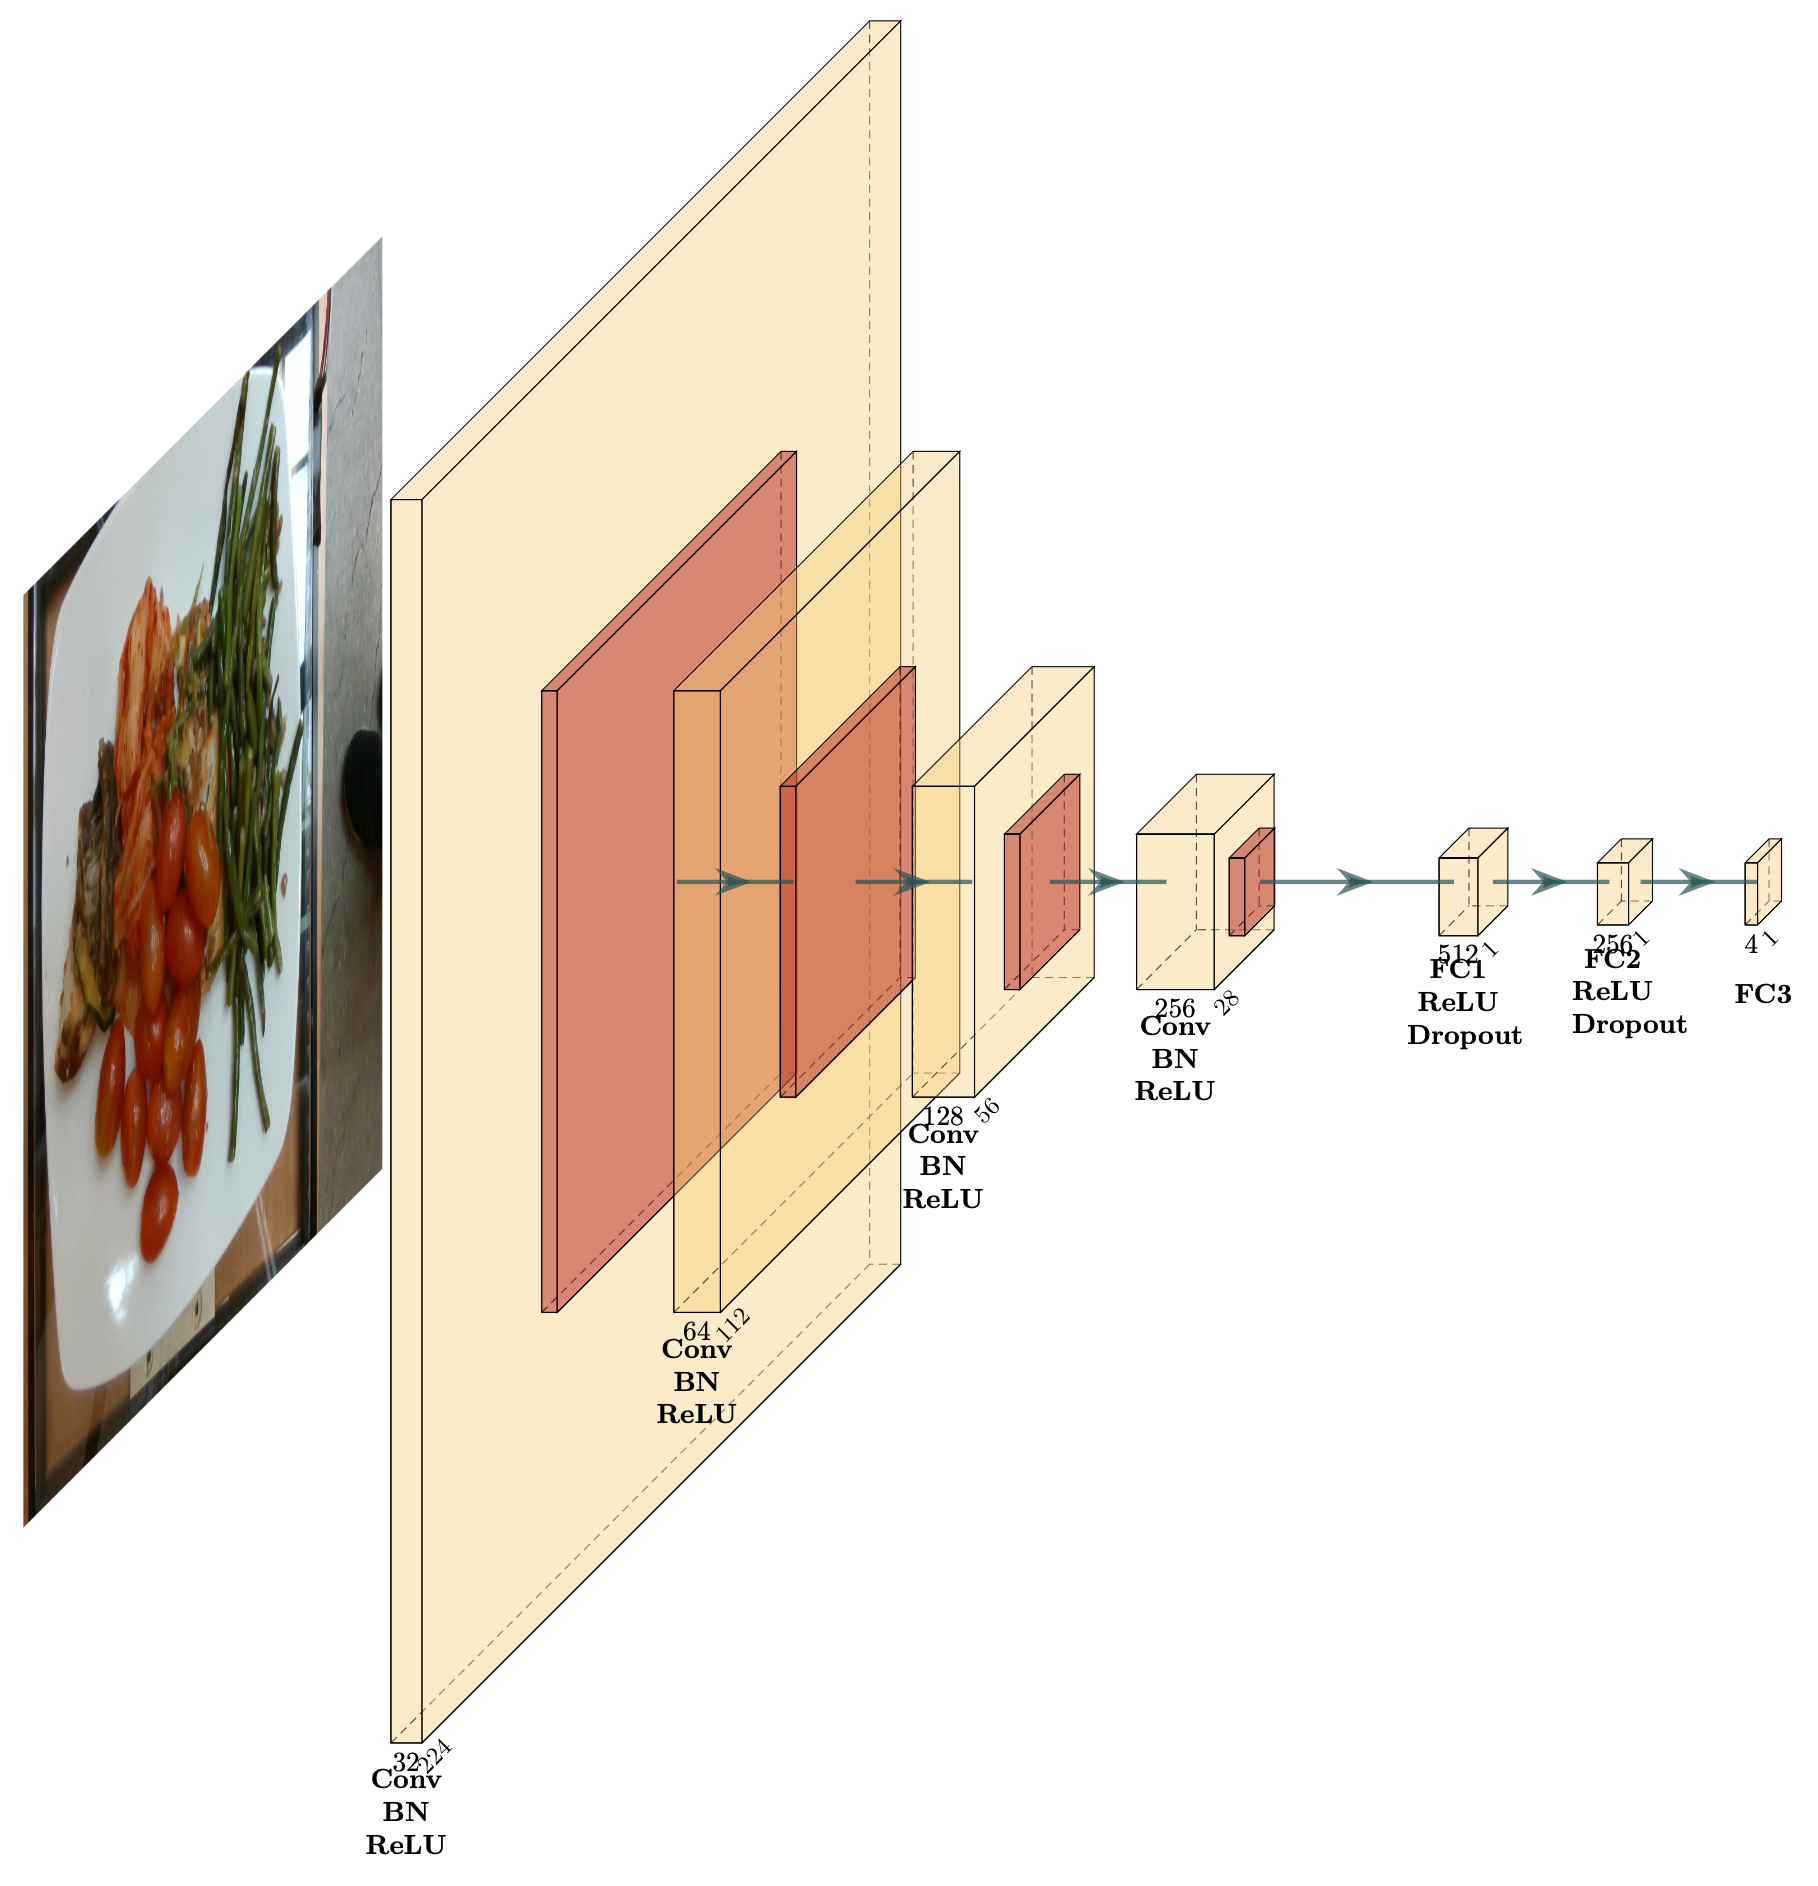
\includegraphics[width=\linewidth, height=3cm]{data/SimpleCNN.png}
%         \caption{Simple CNN}
%         \label{fig:simplecnn_arch}
%     \end{subfigure}
%     \hfill
%     \begin{subfigure}[b]{\textwidth}
%         \centering
%         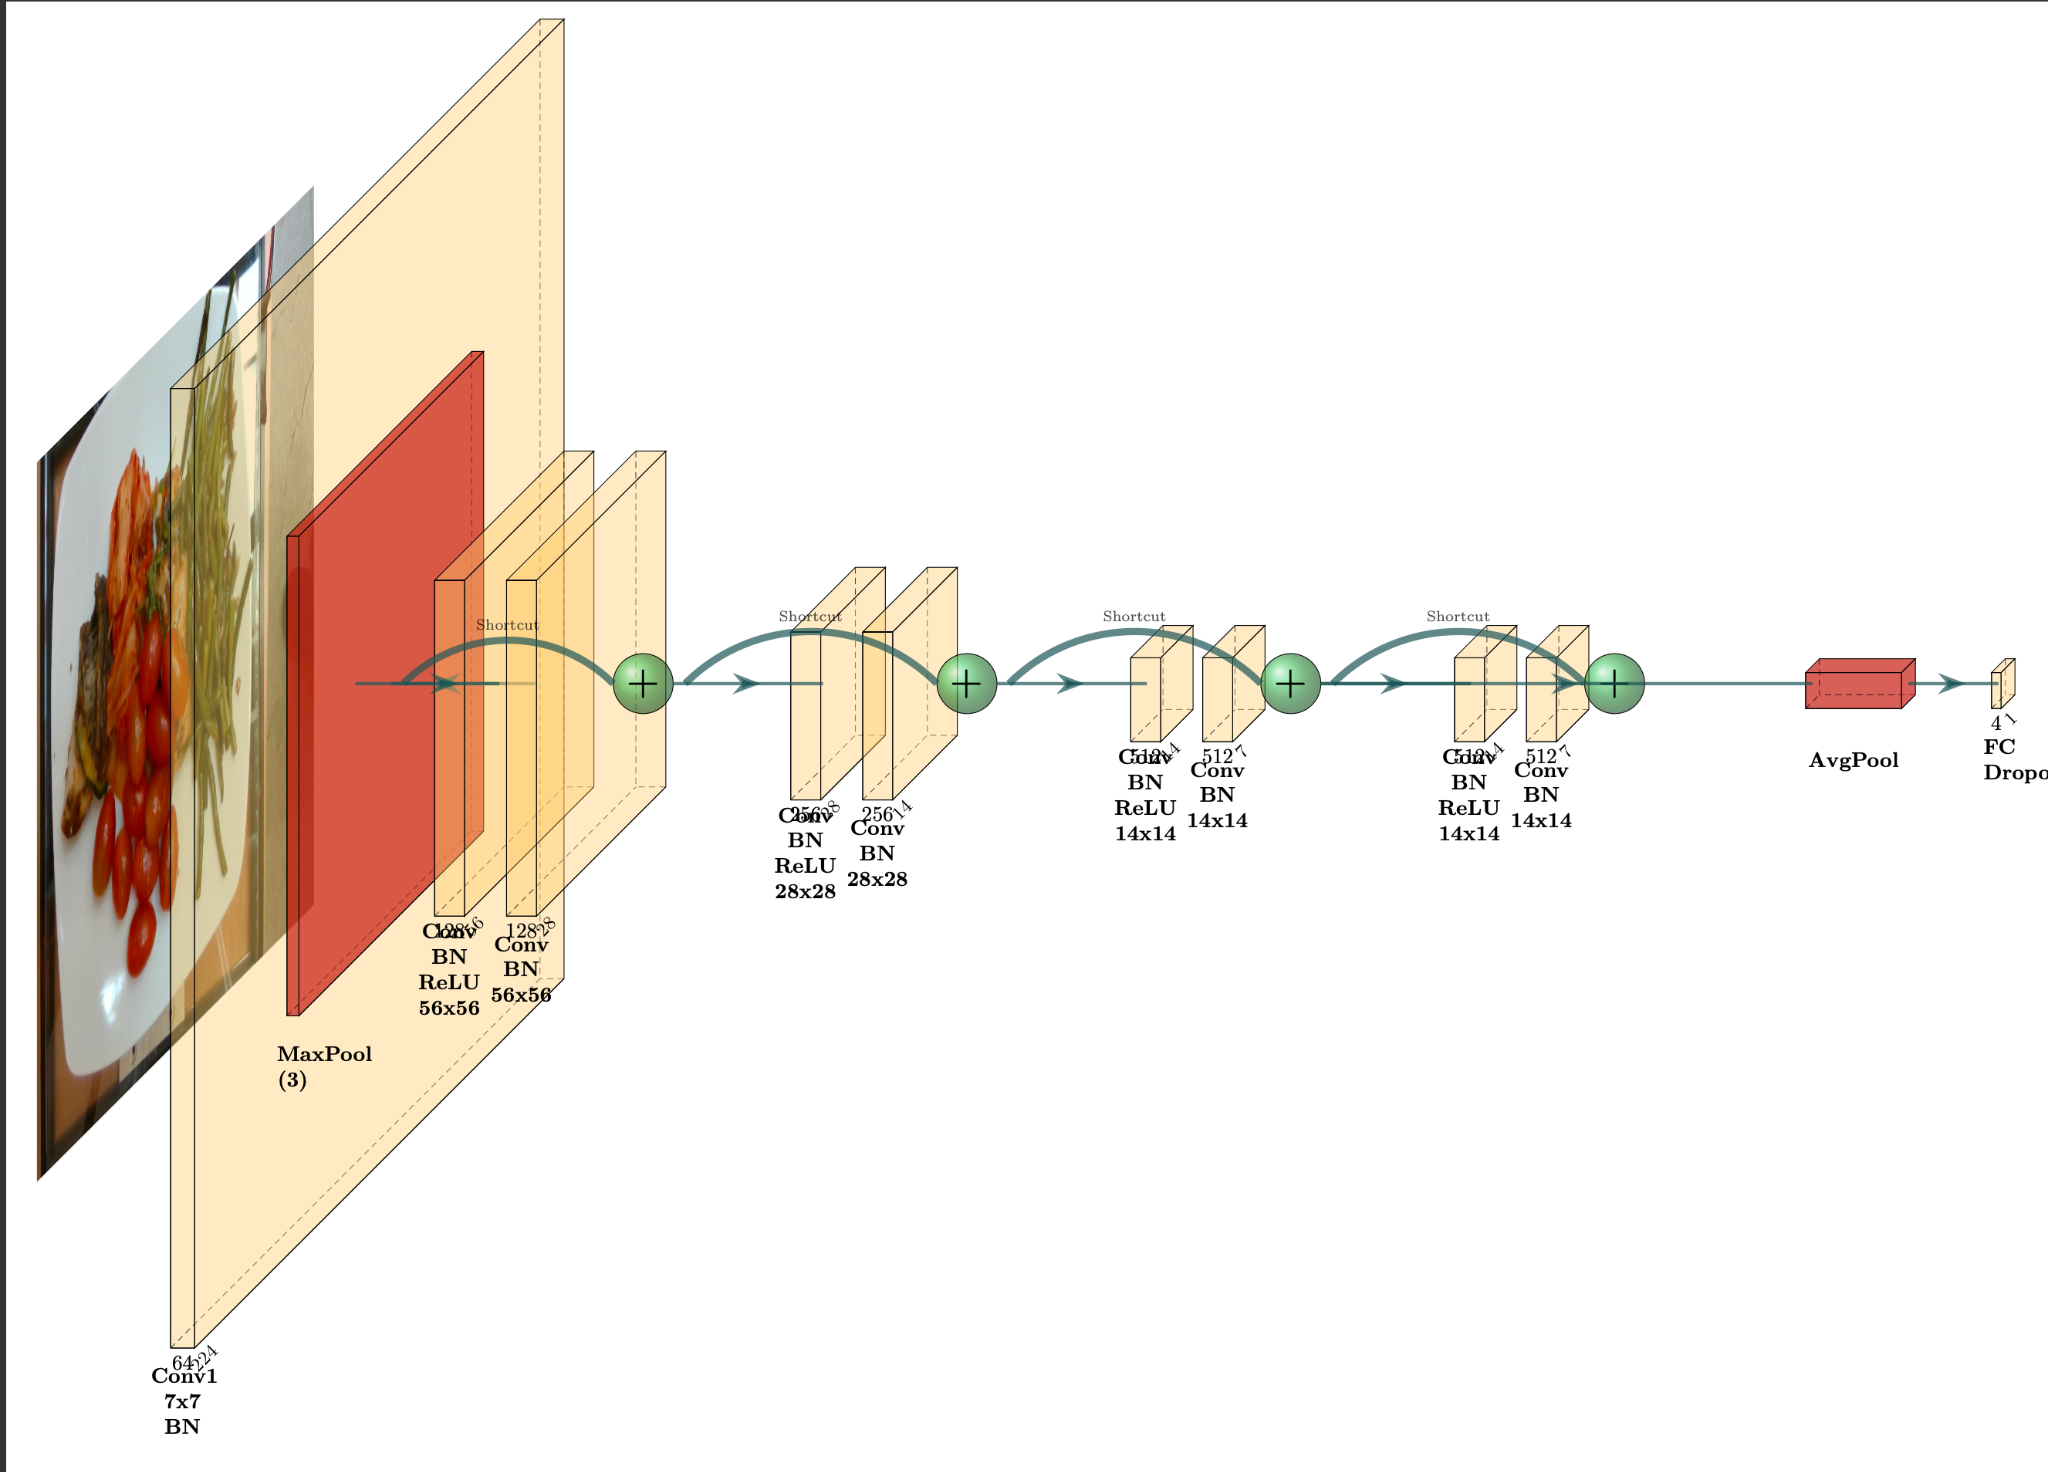
\includegraphics[width=\linewidth, height=3cm]{data/DeepCNN.png}
%         \caption{DeepCNN}
%         \label{fig:deepcnn_arch}
%     \end{subfigure}
    
%     \vspace{1cm} % Add some vertical space between rows
    
%     \begin{subfigure}[b]{\textwidth}
%         \centering
%         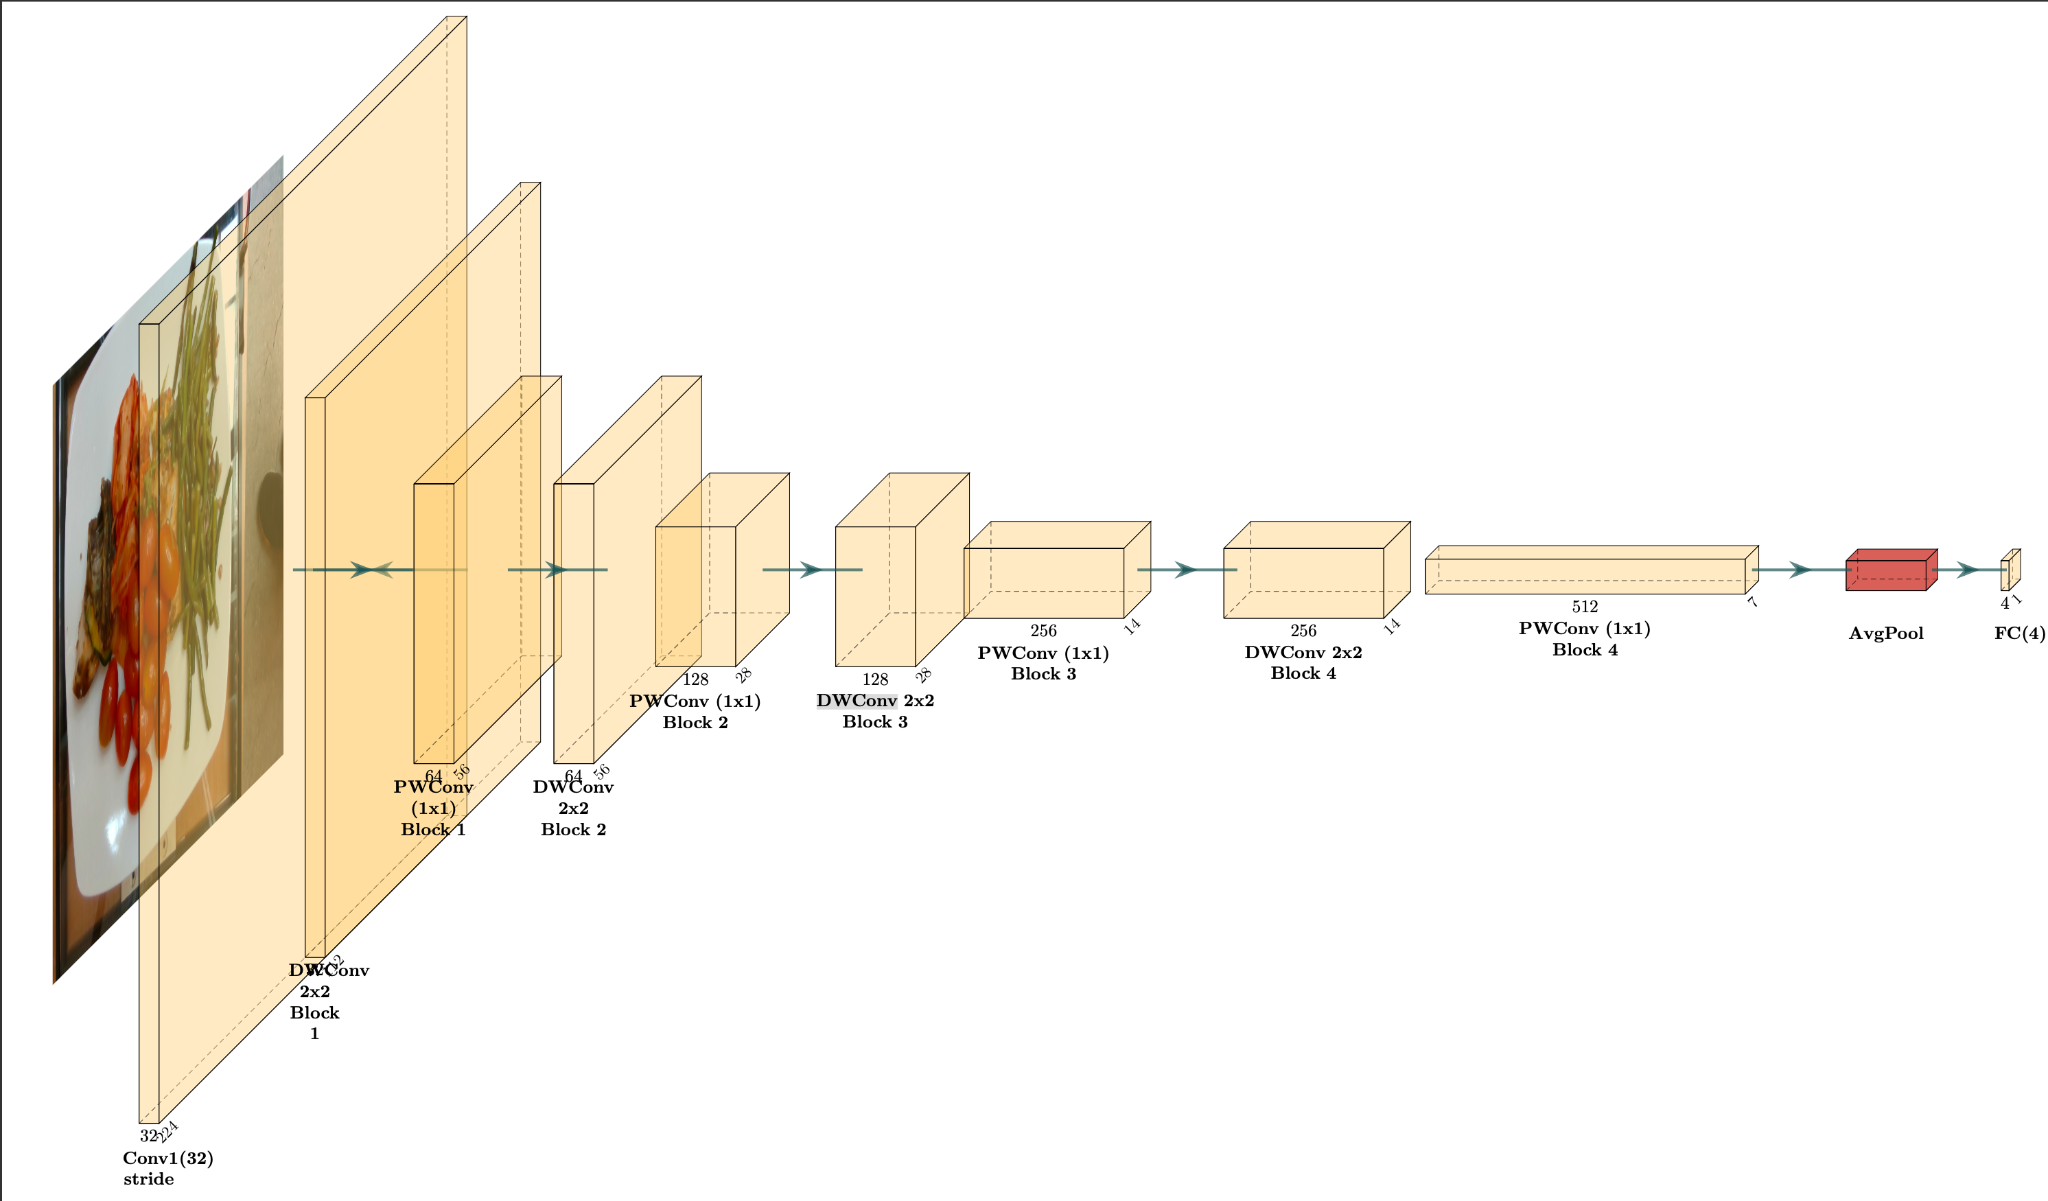
\includegraphics[width=\linewidth, height=3cm]{data/MobileLikeNet.png}
%         \caption{MobileLikeNet}
%         \label{fig:mobilelike_arch}
%     \end{subfigure}
%     \hfill
%     \begin{subfigure}[b]{\textwidth}
%         \centering
%         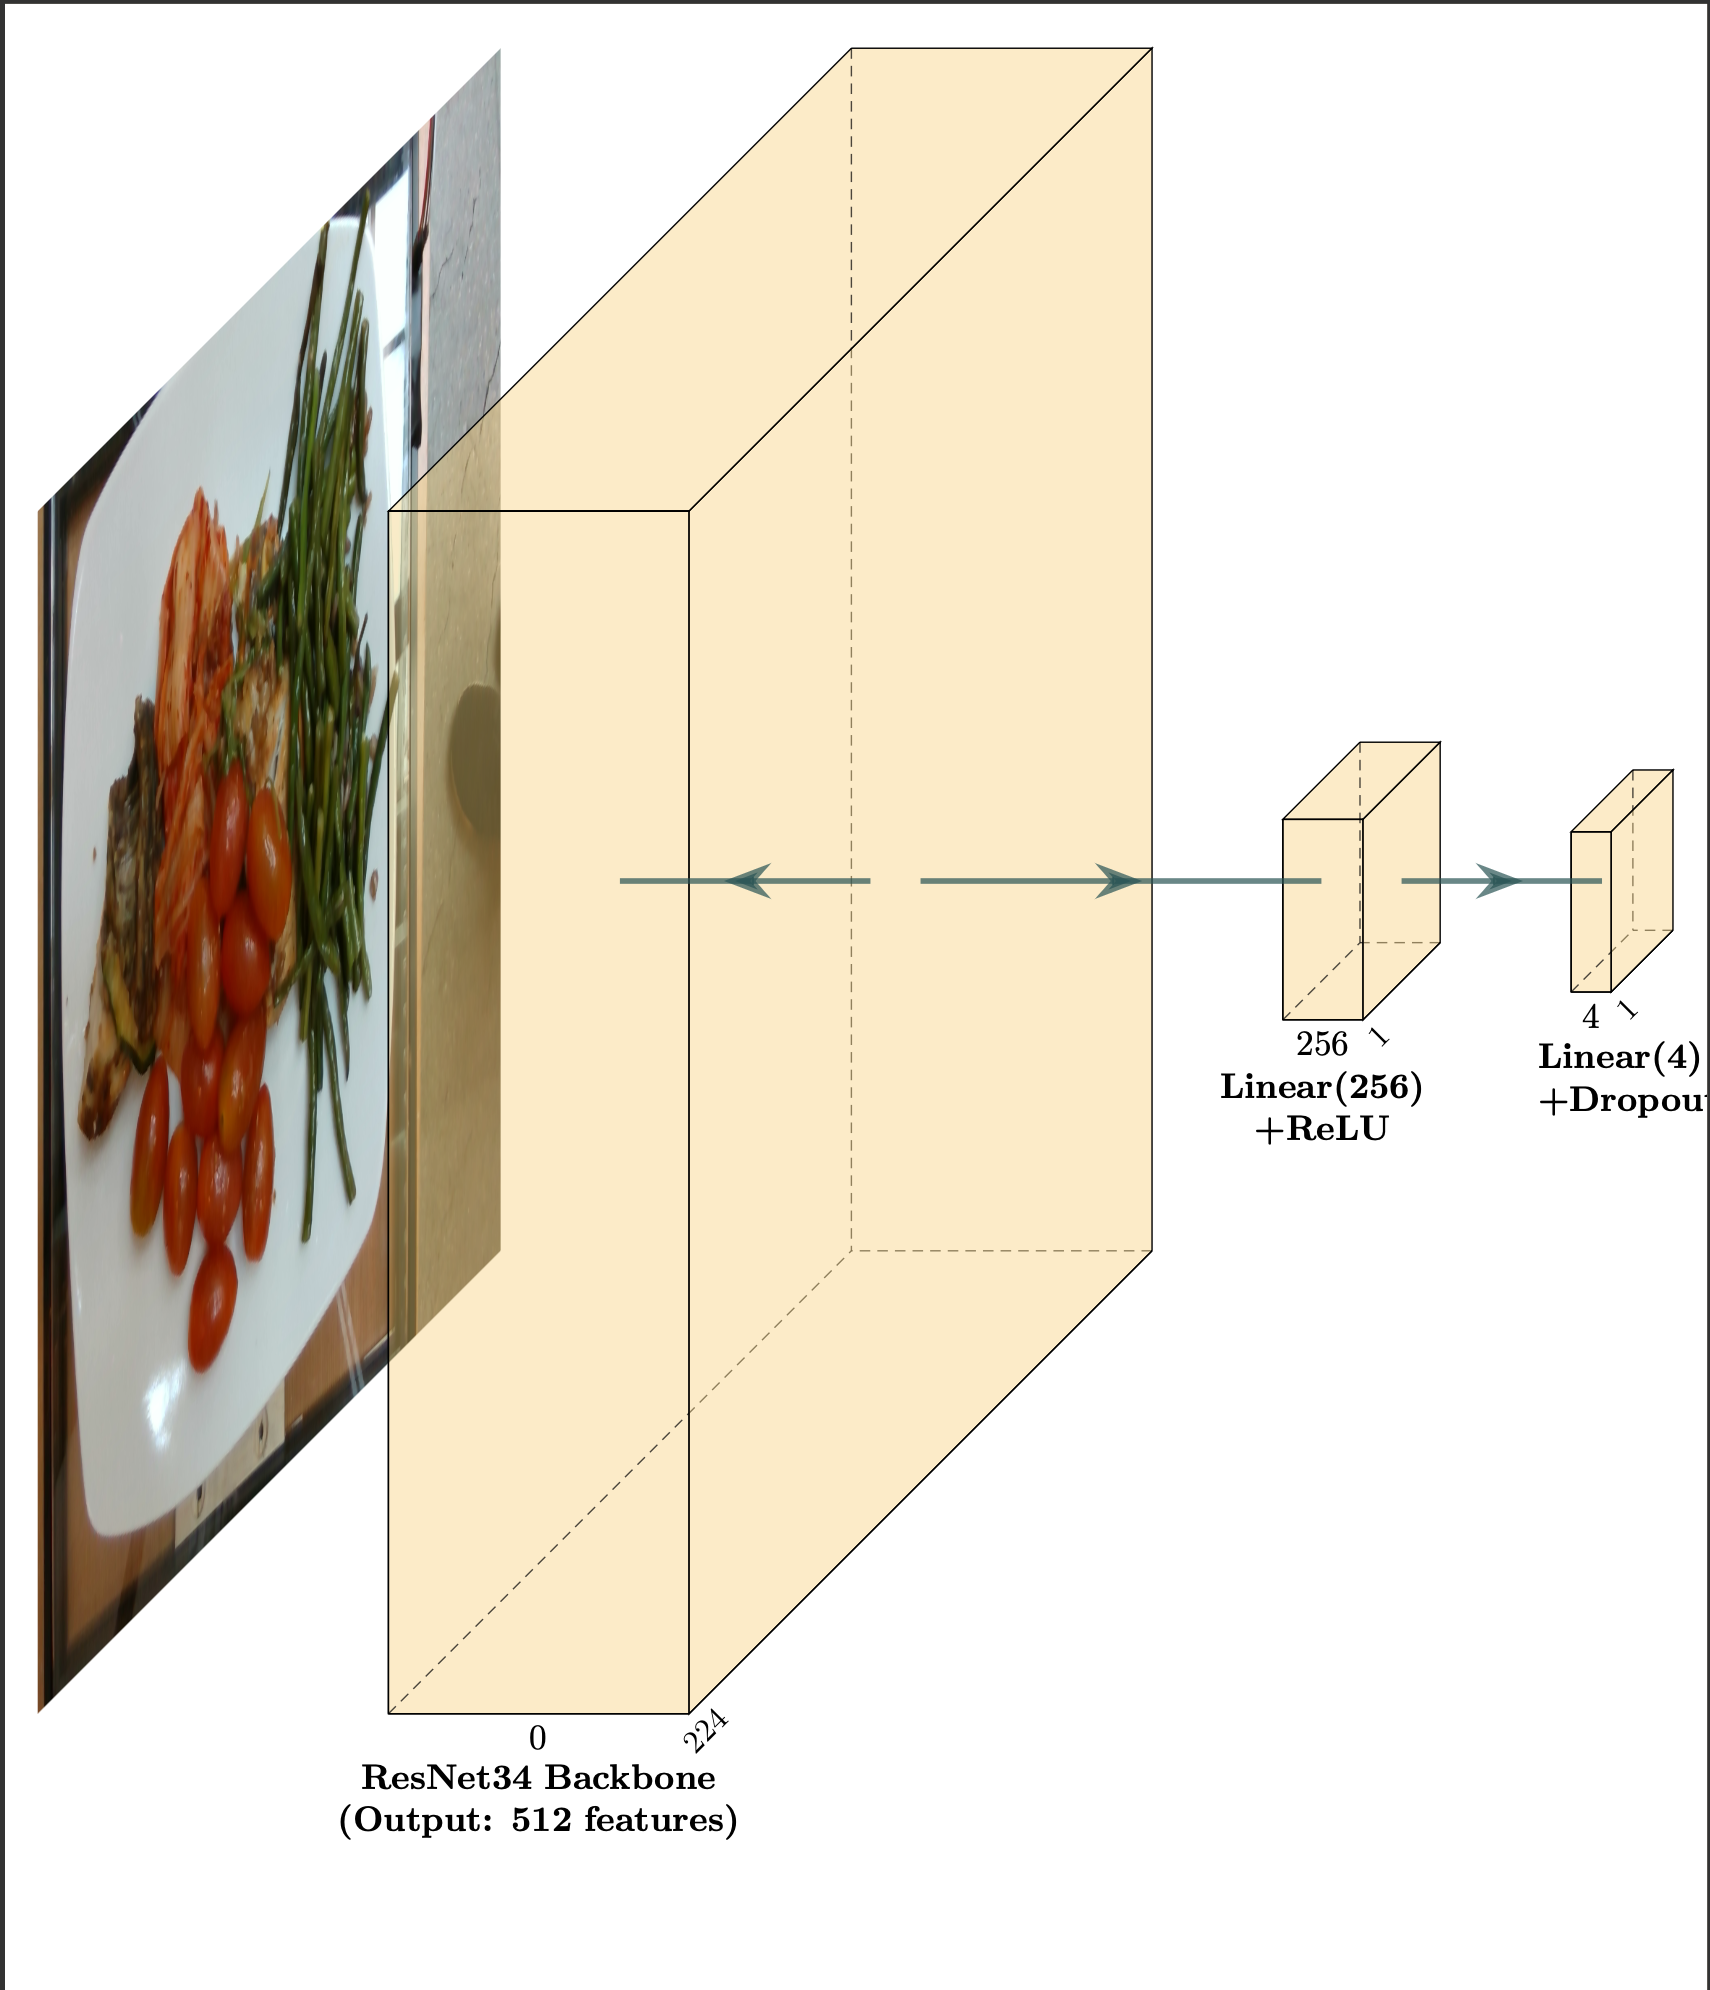
\includegraphics[width=\linewidth, height=3cm]{data/ResNet34.png}
%         \caption{ResNet34}
%         \label{fig:deepcnn_arch}
%     \end{subfigure}
    
%     \caption{Architectures of the four models evaluated. (a) A baseline 4-layer CNN. (b) A deeper 9-layer custom CNN. (c) A lightweight model for mobile applications. (d) A summary of the standard ResNet34 model used.}
%     \label{fig:model_architectures}
% \end{figure}

% TikZ libraries for positioning, arrows, decorations, etc.
\usetikzlibrary{positioning, arrows.meta, calc, decorations.pathreplacing}

\begin{figure}[h!]
\centering
% Resize the whole figure to fit the page width
\resizebox{\textwidth}{!}{%
\begin{tikzpicture}[
    font=\sffamily\small,
    % Define styles for different elements
    tensor_stack/.style={ % Style for the 3D stack of feature maps
        every node/.style={
            draw,
            minimum width=0.5cm,
            minimum height=1.5cm,
            shape=rectangle,
            fill=orange!30,
            opacity=0.8,
            line width=0.5pt
        }
    },
    fc_layer/.style={ % Style for a dense/pooling layer
        draw,
        fill=red!50,
        minimum width=0.2cm,
        minimum height=1cm,
        line width=0.5pt
    },
    label_style/.style={ % Style for text labels
        align=center,
        font=\sffamily\small,
        text width=3cm
    },
    arrow_style/.style={ % Style for arrows between main stages
        -Stealth,
        draw=teal!70!black,
        line width=1.5pt
    },
    brace/.style={ % Style for curly braces
        decorate,
        decoration={brace, amplitude=5pt, raise=2pt},
        line width=0.5pt
    }
]

% --- Define coordinates and place nodes from left to right ---

% 1. INPUT LAYER
\node[draw, minimum size=3cm] (input) {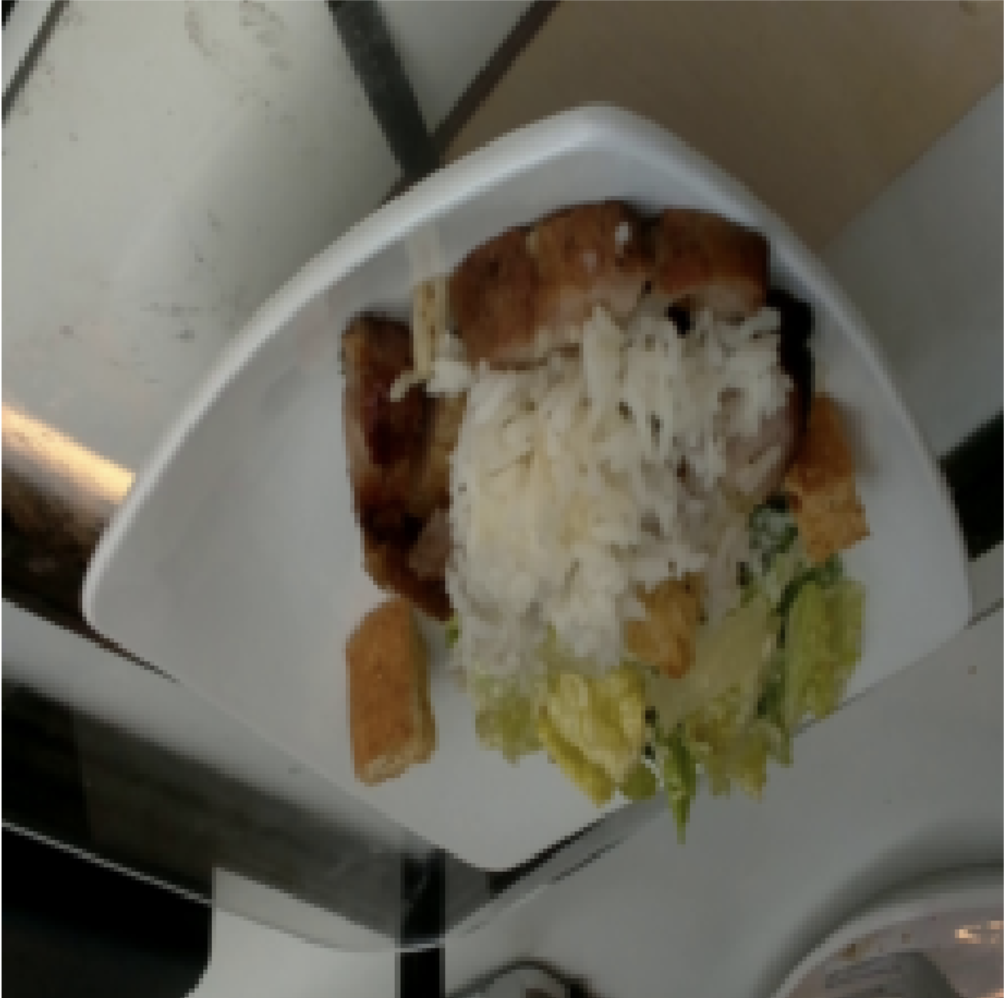
\includegraphics[width=2.8cm]{data/example-food-image.png}};
\node[label_style, text width=2cm, below=0.2cm of input] (input_label) {Input Image};

% Define parameters for the 3D stack illusion
\def\xstackshift{0.08cm}
\def\ystackshift{0.08cm}

% 2. Initial Convolution Layer (Conv1)
\node (conv1_anchor) [right=2cm of input] {};
\begin{scope}[tensor_stack]
    \foreach \i in {1,...,10} {
        \node[minimum height=2.5cm, fill=orange!40, anchor=south west] at ($(conv1_anchor) + (\i*\xstackshift, \i*\ystackshift)$) {};
    }
\end{scope}
\node (conv1_center) at ($(conv1_anchor) + (0.25cm, 1.25cm) + (5*\xstackshift, 5*\ystackshift)$) {};
\node[label_style, below=1.5cm of conv1_center] {Conv1 (32) \\ stride 2};

% --- Feature Extraction Blocks ---

% Helper node for positioning the first block
\node (block1_pos) [right=2.5cm of conv1_center] {};

% Block 1
\node (dw1_anchor) at (block1_pos) {};
\begin{scope}[tensor_stack]
    \foreach \i in {1,...,10} { \node[minimum height=2cm, fill=orange!50, anchor=south west] at ($(dw1_anchor) + (\i*\xstackshift, \i*\ystackshift)$) {}; }
\end{scope}
\node (pw1_anchor) [right=0.5cm of dw1_anchor] {};
\begin{scope}[tensor_stack]
    \foreach \i in {1,...,12} { \node[minimum height=2cm, fill=orange!50, anchor=south west] at ($(pw1_anchor) + (\i*\xstackshift, \i*\ystackshift)$) {}; }
\end{scope}
\node (block1_center) at ($(dw1_anchor) + (0.75cm, 1cm) + (6*\xstackshift, 6*\ystackshift)$) {};
\node[label_style, below=1.5cm of block1_center] {DWConv 2x2, s2 \quad PWConv 1x1 \\ \textbf{Block 1} (64)};

% Block 2
\node (block2_pos) [right=3cm of block1_center] {};
\node (dw2_anchor) at (block2_pos) {};
\begin{scope}[tensor_stack]
    \foreach \i in {1,...,12} { \node[minimum height=1.5cm, fill=orange!60, anchor=south west] at ($(dw2_anchor) + (\i*\xstackshift, \i*\ystackshift)$) {}; }
\end{scope}
\node (pw2_anchor) [right=0.3cm of dw2_anchor] {};
\begin{scope}[tensor_stack]
    \foreach \i in {1,...,14} { \node[minimum height=1.5cm, fill=orange!60, anchor=south west] at ($(pw2_anchor) + (\i*\xstackshift, \i*\ystackshift)$) {}; }
\end{scope}
\node (block2_center) at ($(dw2_anchor) + (0.9cm, 0.75cm) + (7*\xstackshift, 7*\ystackshift)$) {};
\node[label_style, below=1.2cm of block2_center] {DWConv 2x2, s2 \quad PWConv 1x1 \\ \textbf{Block 2} (128)};

% Block 3
\node (block3_pos) [right=3.5cm of block2_center] {};
\node (dw3_anchor) at (block3_pos) {};
\begin{scope}[tensor_stack]
    \foreach \i in {1,...,14} { \node[minimum height=1.0cm, fill=orange!70, anchor=south west] at ($(dw3_anchor) + (\i*\xstackshift, \i*\ystackshift)$) {}; }
\end{scope}
\node (pw3_anchor) [right=0.4cm of dw3_anchor] {};
\begin{scope}[tensor_stack]
    \foreach \i in {1,...,16} { \node[minimum height=1.0cm, fill=orange!70, anchor=south west] at ($(pw3_anchor) + (\i*\xstackshift, \i*\ystackshift)$) {}; }
\end{scope}
\node (block3_center) at ($(dw3_anchor) + (1.2cm, 0.5cm) + (8*\xstackshift, 8*\ystackshift)$) {};
\node[label_style, below=1.2cm of block3_center] {DWConv 2x2, s2 \quad PWConv 1x1 \\ \textbf{Block 3} (256)};

% Block 4
\node (block4_pos) [right=4cm of block3_center] {};
\node (dw4_anchor) at (block4_pos) {};
\begin{scope}[tensor_stack]
    \foreach \i in {1,...,16} { \node[minimum height=0.75cm, fill=orange!80, anchor=south west] at ($(dw4_anchor) + (\i*\xstackshift, \i*\ystackshift)$) {}; }
\end{scope}
\node (pw4_anchor) [right=0.5cm of dw4_anchor] {};
\begin{scope}[tensor_stack]
    \foreach \i in {1,...,18} { \node[minimum height=0.75cm, fill=orange!80, anchor=south west] at ($(pw4_anchor) + (\i*\xstackshift, \i*\ystackshift)$) {}; }
\end{scope}
\node (block4_center) at ($(dw4_anchor) + (1.4cm, 0.375cm) + (9*\xstackshift, 9*\ystackshift)$) {};
\node[label_style, below=1.0cm of block4_center] {DWConv 2x2, s2 \quad PWConv 1x1 \\ \textbf{Block 4} (512)};

% 4. Classifier/Regressor Head
\node[fc_layer, right=3cm of block4_center] (avg_pool) {};
\node[label_style, text width=2cm, below=0.2cm of avg_pool] {AvgPool};

\node[fc_layer, right=1.5cm of avg_pool, minimum height=1.5cm] (output_vec) {};
\node[label_style, text width=2cm, below=0.55cm of output_vec] {Output \\ Vector};

% --- Output Labels ---
\node[align=left, right=0.5cm of output_vec] (output_labels) {
    Calories / 100g \\
    Proteins / 100g \\
    Carbs / 100g \\
    Fats / 100g
};
% Add a brace to group the outputs
\draw[brace] ($(output_labels.north east)+(0.1,0.1)$) -- node[right=5pt] {OUTPUT} ($(output_labels.south east)+(0.1,-0.1)$);

% --- Draw Connections Between Layers ---
\draw[arrow_style] (input.east) -- (conv1_center);
\draw[arrow_style] (conv1_center) -- (block1_center);
\draw[arrow_style] (block1_center) -- (block2_center);
\draw[arrow_style] (block2_center) -- (block3_center);
\draw[arrow_style] (block3_center) -- (block4_center);
\draw[arrow_style] (block4_center) -- (avg_pool.west);
\draw[arrow_style] (avg_pool.east) -- (output_vec.west);

\end{tikzpicture}
} % end \resizebox
\caption{Mobile-Like Net}
\label{fig:nutritional_cnn_architecture}
\end{figure}

\begin{figure}[h!]
\centering
% Resize the whole figure to fit the page width
\resizebox{\textwidth}{!}{%
\begin{tikzpicture}[
    font=\sffamily\small,
    % Define styles for different elements
    tensor_stack/.style={ % Style for the 3D stack of feature maps
        every node/.style={
            draw,
            minimum width=0.4cm,
            minimum height=1.2cm,
            shape=rectangle,
            fill=orange!30,
            opacity=0.8,
            line width=0.5pt
        }
    },
    sum_circle/.style={
        circle,
        draw,
        fill=green!60,
        minimum size=8mm,
        inner sep=0pt
    },
    fc_layer/.style={ % Style for a dense/pooling layer
        draw,
        fill=red!50,
        minimum width=0.2cm,
        minimum height=1cm,
        line width=0.5pt
    },
    label_style/.style={ % Style for text labels
        align=center,
        font=\sffamily\small
    },
    arrow_style/.style={ % Style for arrows between main stages
        -Stealth,
        draw=teal!70!black,
        line width=1.5pt
    },
    brace/.style={ % Style for curly braces
        decorate,
        decoration={brace, amplitude=5pt, raise=2pt},
        line width=0.5pt
    }
]

% Define parameters for the 3D stack illusion
\def\xstackshift{0.08cm}
\def\ystackshift{0.08cm}

% --- Place Nodes from Left to Right ---

% 1. INPUT LAYER
\node[draw, minimum size=3cm] (input) {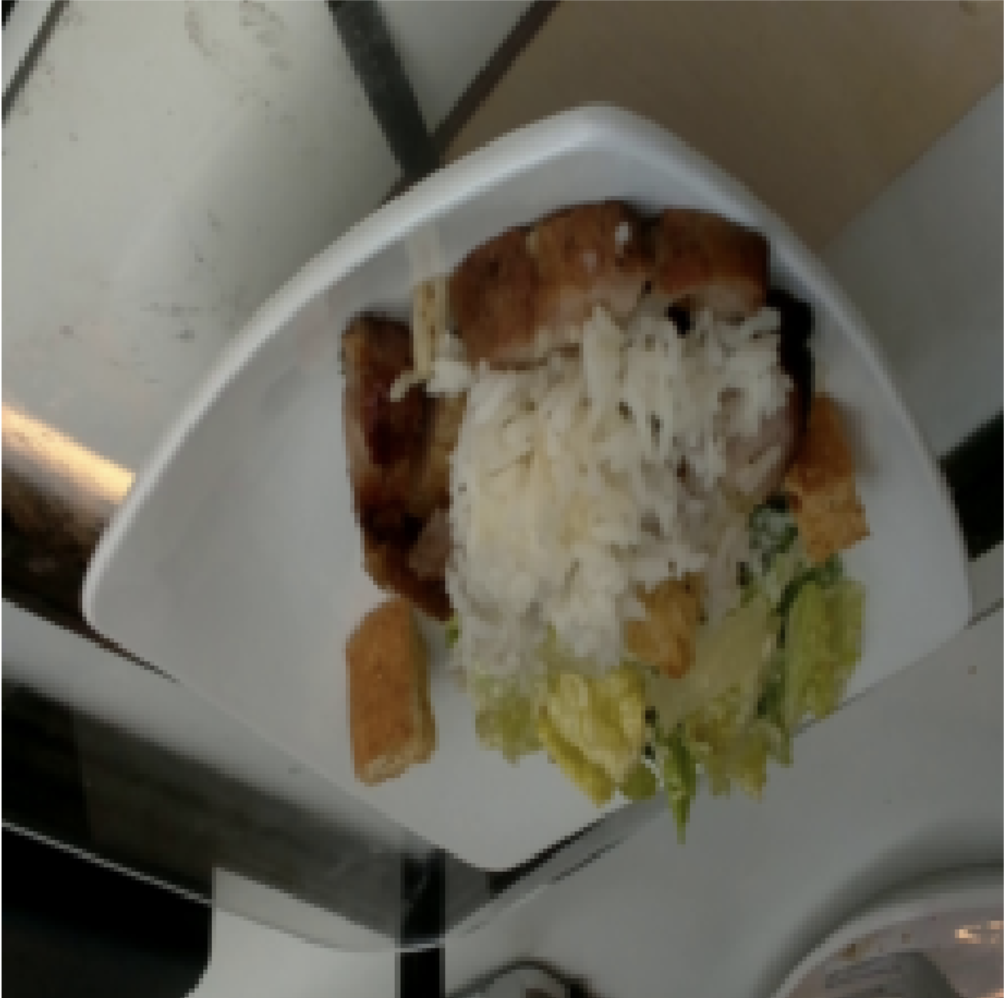
\includegraphics[width=2.8cm]{data/example-food-image.png}};
\node[label_style, text width=2cm, below=0.2cm of input] {Input Image};

% 2. Initial Convolution Block
\node (conv1_anchor) [right=1.5cm of input] {};
\begin{scope}[tensor_stack]
    \foreach \i in {1,...,10} {
        \node[minimum height=2.5cm, fill=orange!40, anchor=south west] at ($(conv1_anchor) + (\i*\xstackshift, \i*\ystackshift)$) {};
    }
\end{scope}
\node (conv1_center) at ($(conv1_anchor) + (0.2cm, .5cm) + (5*\xstackshift, 5*\ystackshift)$) {};
\node[label_style, text width=2.5cm, below=1.5cm of conv1_center] {7x7 Conv, BN \\ MaxPool \\ (56x56)};

% --- Residual Blocks ---

% Helper node to start the residual chain
\node (res_start) [right=1.5cm of conv1_center] {};
\coordinate (in_node) at (res_start); % Start with the output of Conv1

% Loop to create the residual blocks
\foreach \i in {1, 2, 3, 4} {
    % *** FIXED CODE: Calculate dimensions and store in macros ***
    \pgfmathsetmacro{\blockheight}{1.8 - 0.45*\i}
    \pgfmathsetmacro{\blockycenter}{\blockheight/2}
    
    % Main path blocks
    \node (block\i a_anchor) [right=1cm of in_node] {};
    \begin{scope}[tensor_stack]
        \foreach \k in {1,...,8} {\node[minimum height=\blockheight cm, anchor=south west] at ($(block\i a_anchor) + (\k*\xstackshift, \k*\ystackshift)$) {};}
    \end{scope}
    \node (block\i a_center) at ($(block\i a_anchor) + (0.2cm, \blockycenter cm) + (2*\xstackshift, 2*\ystackshift)$) {};

    \node (block\i b_anchor) [right=0.5cm of block\i a_center] {};
    \begin{scope}[tensor_stack]
        \foreach \k in {1,...,8} {\node[minimum height=\blockheight cm, anchor=south west] at ($(block\i b_anchor) + (\k*\xstackshift, \k*\ystackshift)$) {};}
    \end{scope}
    \node (block\i b_center) at ($(block\i b_anchor) + (0.2cm, \blockycenter cm) + (2*\xstackshift, 2*\ystackshift)$) {};

    % Summation Circle
    \node[sum_circle, right=0.7cm of block\i b_center] (sum\i) {+};

    % Main path arrows
    \draw[arrow_style] (in_node) -- (block\i a_center);
    \draw[arrow_style] (block\i a_center) -- (block\i b_center);
    \draw[arrow_style] (block\i b_center) -- (sum\i);

    % Shortcut path arrow
    \draw[arrow_style, rounded corners] (in_node) .. controls +(0,1.5) and +(-1.5,1.5) .. (sum\i.north);
    \node[label_style, font=\tiny, above=-1.5cm of $(in_node)!0.5!(sum\i)$] {Shortcut};
    
    % Update the input node for the next iteration
    \coordinate (in_node) at (sum\i);
}

% --- Classifier/Regressor Head ---
\node[fc_layer, right=1.5cm of in_node] (avg_pool) {};
\node[label_style, text width=2cm, below=0.2cm of avg_pool] {AvgPool};

\node[fc_layer, right=1cm of avg_pool, minimum height=1.5cm] (output_vec) {};

% --- Output Labels ---
\node[align=left, right=0.5cm of output_vec] (output_labels) {
    Calories / 100g \\
    Proteins / 100g \\
    Carbs / 100g \\
    Fats / 100g
};
% Add a brace to group the outputs
\draw[brace] ($(output_labels.north east)+(0.1,0.1)$) -- node[right=5pt] {OUTPUT} ($(output_labels.south east)+(0.1,-0.1)$);

% --- Final Connections ---
\draw[arrow_style] (input.east) -- (conv1_center);
\draw[arrow_style] (conv1_center) -- (res_start);
\draw[arrow_style] (in_node) -- (avg_pool.west);
\draw[arrow_style] (avg_pool.east) -- (output_vec.west);

\end{tikzpicture}
} % end \resizebox
\caption{Deep CNN}
\label{fig:resnet_nutrition_architecture}
\end{figure}

\begin{figure}[hbt!]
\centering
% Resize the whole figure to fit the page width
\resizebox{\textwidth}{!}{%
\begin{tikzpicture}[
    font=\sffamily\small,
    % Define styles for different elements
    tensor_stack/.style={ % Style for the 3D stack of feature maps
        every node/.style={
            draw,
            minimum width=0.5cm,
            shape=rectangle,
            fill=orange!30,
            opacity=0.8,
            line width=0.5pt
        }
    },
    fc_layer/.style={ % Style for a dense/pooling layer
        draw,
        fill=orange!60,
        minimum width=0.2cm,
        minimum height=1.2cm,
        line width=0.5pt
    },
    label_style/.style={ % Style for text labels
        align=center,
        font=\sffamily\small
    },
    arrow_style/.style={ % Style for arrows between main stages
        -Stealth,
        draw=teal!70!black,
        line width=1.5pt
    },
    brace/.style={ % Style for curly braces
        decorate,
        decoration={brace, amplitude=5pt, raise=2pt},
        line width=0.5pt
    }
]

% Define parameters for the 3D stack illusion
\def\xstackshift{0.08cm}
\def\ystackshift{0.08cm}

% --- Place Nodes from Left to Right ---

% 1. INPUT LAYER
\node[draw, minimum size=3.5cm] (input) {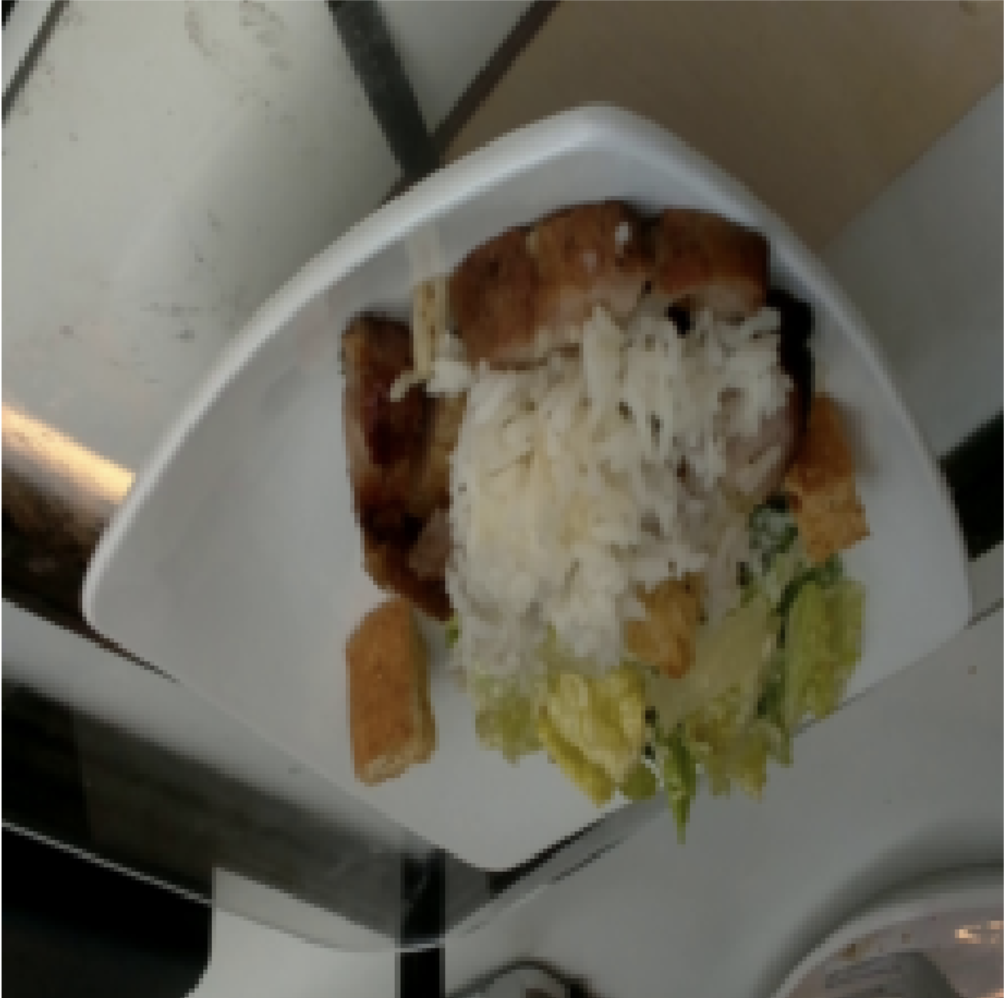
\includegraphics[width=3.3cm]{data/example-food-image.png}};
\node[label_style, text width=2cm, below=0.2cm of input] {Input Image};

% --- Convolutional Blocks ---

% Conv Block 1 (32 channels, ~112x112)
\node (conv1_anchor) [right=1.5cm of input] {};
\begin{scope}[tensor_stack]
    \foreach \i in {1,...,8} { \node[minimum height=3.0cm, fill=orange!30, anchor=south west] at ($(conv1_anchor) + (\i*\xstackshift, \i*\ystackshift)$) {}; }
\end{scope}
\node (conv1_center) at ($(conv1_anchor) + (0.2cm, 1.0cm) + (2*\xstackshift, 2*\ystackshift)$) {};
\node[label_style, text width=2.5cm, below=1.5cm of conv1_center] {Conv (32) \\ BN, ReLU};

% Conv Block 2 (64 channels, 112x112)
\node (conv2_anchor) [right=1.5cm of conv1_center] {};
\begin{scope}[tensor_stack]
    \foreach \i in {1,...,10} { \node[minimum height=3.0cm, fill=orange!40, anchor=south west] at ($(conv2_anchor) + (\i*\xstackshift, \i*\ystackshift)$) {}; }
\end{scope}
\node (conv2_center) at ($(conv2_anchor) + (0.25cm, 1.0cm) + (2*\xstackshift, 2*\ystackshift)$) {};
\node[label_style, text width=2.5cm, below=1.8cm of conv2_center] {Conv (64) \\ BN, ReLU \\ 112x112};

% Conv Block 3 (128 channels, 56x56)
\node (conv3_anchor) [right=2cm of conv2_center] {};
\begin{scope}[tensor_stack]
    \foreach \i in {1,...,12} { \node[minimum height=2.0cm, fill=orange!50, anchor=south west] at ($(conv3_anchor) + (\i*\xstackshift, \i*\ystackshift)$) {}; }
\end{scope}
\node (conv3_center) at ($(conv3_anchor) + (0.3cm, 1.0cm) + (6*\xstackshift, 6*\ystackshift)$) {};
\node[label_style, text width=2.5cm, below=1.5cm of conv3_center] {Conv (128) \\ BN, ReLU \\ 56x56};

% Conv Block 4 (256 channels, 28x28)
\node (conv4_anchor) [right=2.5cm of conv3_center] {};
\begin{scope}[tensor_stack]
    \foreach \i in {1,...,14} { \node[minimum height=1.0cm, fill=orange!60, anchor=south west] at ($(conv4_anchor) + (\i*\xstackshift, \i*\ystackshift)$) {}; }
\end{scope}
\node (conv4_center) at ($(conv4_anchor) + (0.35cm, 0.5cm) + (7*\xstackshift, 7*\ystackshift)$) {};
\node[label_style, text width=2.5cm, below=0.8cm of conv4_center] {Conv (256) \\ BN, ReLU \\ 28x28};


% --- Fully Connected (FC) Layers ---
\node[fc_layer, right=2.5cm of conv4_center] (fc1) {};
\node[label_style, text width=2cm, below=0.2cm of fc1] {FC1 (512) \\ ReLU \\ Dropout};

\node[fc_layer, right=1.5cm of fc1] (fc2) {};
\node[label_style, text width=2cm, below=0.2cm of fc2] {FC2 (256) \\ ReLU \\ Dropout};

% --- Output Layer ---
\node[fc_layer, right=1.5cm of fc2, minimum height=0.8cm] (output_vec) {};
\node[align=left, right=0.5cm of output_vec] (output_labels) {
    Calories / 100g \\
    Proteins / 100g \\
    Carbs / 100g \\
    Fats / 100g
};
% Add a brace to group the outputs
\draw[brace] ($(output_labels.north east)+(0.1,0.1)$) -- node[right=5pt] {OUTPUT} ($(output_labels.south east)+(0.1,-0.1)$);

% --- Draw Connections Between Layers ---
\draw[arrow_style] (input.east) -- (conv1_center);
\draw[arrow_style] (conv1_center) -- (conv2_center);
\draw[arrow_style] (conv2_center) -- (conv3_center);
\draw[arrow_style] (conv3_center) -- (conv4_center);
\draw[arrow_style] (conv4_center) -- (fc1);
\draw[arrow_style] (fc1) -- (fc2);
\draw[arrow_style] (fc2) -- (output_vec);

\end{tikzpicture}
} % end \resizebox
\caption{SimpleCNN}
\label{fig:sequential_cnn_architecture}
\end{figure}

\begin{figure}[h!]
\centering
% Resize the whole figure to fit the page width
\resizebox{\textwidth}{!}{%
\begin{tikzpicture}[
    font=\sffamily\small,
    % Define styles for different elements
    backbone_style/.style={ % Style for the large backbone
        draw,
        fill=orange!20,
        minimum width=3cm,
        minimum height=6cm,
        line width=0.5pt
    },
    fc_layer/.style={ % Style for a dense/pooling layer
        draw,
        fill=orange!40,
        minimum width=0.8cm,
        minimum height=2cm,
        line width=0.5pt
    },
    label_style/.style={ % Style for text labels
        align=center,
        font=\sffamily\small
    },
    arrow_style/.style={ % Style for arrows between main stages
        -Stealth,
        draw=teal!70!black,
        line width=1.5pt
    },
    brace/.style={ % Style for curly braces
        decorate,
        decoration={brace, amplitude=5pt, raise=2pt},
        line width=0.5pt
    }
]

% --- Place Nodes from Left to Right ---

% 1. INPUT LAYER
\node[draw, minimum size=4cm] (input) {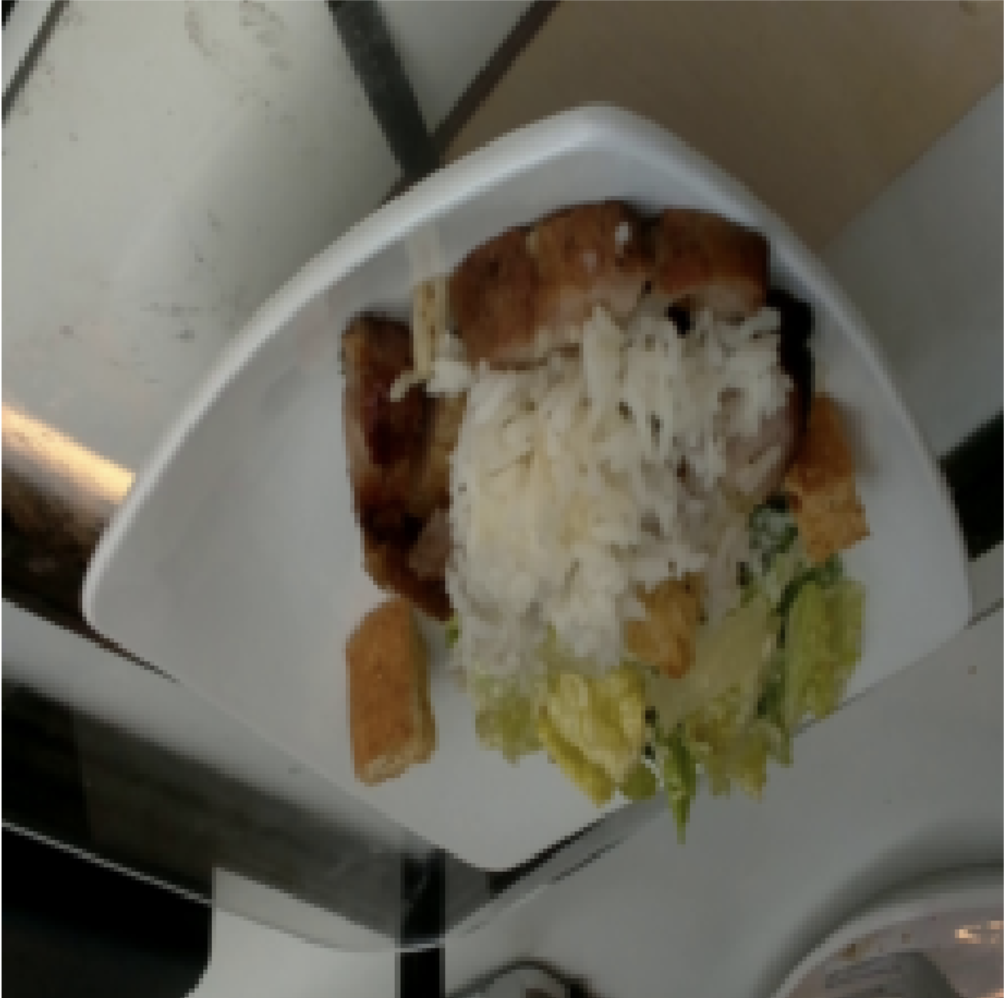
\includegraphics[width=3.8cm]{data/example-food-image.png}};
\node[label_style, text width=2cm, below=0.2cm of input] {Input Image};

% 2. ResNet34 Backbone
% We draw a simple rectangle for the backbone. It's more reliable.
\node[backbone_style, right=2cm of input] (backbone) {};
\node[label_style, text width=4cm, below=0.2cm of backbone] {ResNet34 Backbone \\ (Output: 512 features)};
% To give a slight 3D effect, we can draw a dashed rectangle behind it.
\draw[dashed, thin] ($(backbone.north west)+(0.8cm,0.8cm)$) -- ($(backbone.north east)+(0.8cm,0.8cm)$) -- ($(backbone.south east)+(0.8cm,0.8cm)$);
\draw[dashed, thin] ($(backbone.north east)$) -- ($(backbone.north east)+(0.8cm,0.8cm)$);
\draw[dashed, thin] ($(backbone.south east)$) -- ($(backbone.south east)+(0.8cm,0.8cm)$);

\draw[dashed, thin] ($(backbone.north west)$) -- ($(backbone.north west)+(0.8cm,0.8cm)$);

% --- Custom Head ---

% 3. First Linear Layer
\node[fc_layer, right=3cm of backbone] (linear1) {};
\node[label_style, text width=3cm, below=0.2cm of linear1] {Linear (256) \\ +ReLU};

% 4. Second Linear Layer (Output)
\node[fc_layer, right=2cm of linear1, minimum height=1.5cm, minimum width=0.4cm] (linear2) {};

% --- Output Labels ---
\node[align=left, right=0.8cm of linear2] (output_labels) {
    Calories / 100g \\
    Proteins / 100g \\
    Carbs / 100g \\
    Fats / 100g
};
% Add a brace to group the outputs
\draw[brace] ($(output_labels.north east)+(0.1,0.1)$) -- node[right=5pt] {OUTPUT} ($(output_labels.south east)+(0.1,-0.1)$);

% --- Draw Connections Between Layers ---
\draw[arrow_style] (input.east) -- (backbone.west);
\draw[arrow_style] (backbone.east) -- (linear1.west);
\draw[arrow_style] (linear1.east) -- (linear2.west);
\draw[arrow_style] (linear2.east) -- (output_labels.west);


\end{tikzpicture}
} % end \resizebox
\caption{A pre-trained ResNet34 backbone}
\label{fig:transfer_learning_architecture}
\end{figure}


        
        \subsubsection{SimpleCNN}
            For the purpose of better understanding the problem and simplicity we start with so-called SimpleCNN which is essentially a 4-layer Convolution Network. 

            Figure \ref{fig:sequential_cnn_architecture} serves as our baseline.(\textit{LR: 1e-3, Params: 26.2M}).

            \subsubsection{DeepCNN}
            To push our capabilities to the maximum we explore DeepCNN model - Deep Convolution Neural Network to try to achieve the best results without pre-trained models. 
            
            9 Convolution layers, followed by average pooling layer and fully-connected layer (Figure \ref{fig:resnet_nutrition_architecture}) .(\textit{LR: 1e-4, Params: 9.8M}). Surprisingly, the results seem to be the same as for Simple CNN, maybe because of the early stopping we couldn't fully exploit deep cnn abilities. 

        \subsubsection{MobileLikeNet}{
            Our third explored model is user-oriented, since calories estimation is prominent topic and demand for accurate solutions is very high, we explore applied models that can be installed on phones and mobile devices. One such model would be MoblileLike Network - light CNN that is not computationally heavy. 
            (\textit{LR: 1e-4, Params: 184k}).
        }

        \subsubsection{ResNet34}
        {
            (Figure \ref{fig:transfer_learning_architecture}) is a standard, very deep architecture pre-trained on ImageNet. We fine-tuned it for our regression task. (\textit{LR: 1e-5, Params: 21.4M}).
        }
        \subsection{Percentage estimation results}
        \begin{table}[hbt!]
\centering
\caption{Performance Metrics of Different CNN Models for Nutrient Estimation. Best values are in \textbf{bold}.}
\label{tab:combined_results_booktabs}
\small
\begin{tabular}{llrrrrrrrr}
\toprule
& & \multicolumn{4}{c}{Extended dataset} & \multicolumn{4}{c}{Original dataset} \\
\cmidrule(lr){3-6} \cmidrule(l){7-10}
\textbf{Model} & \textbf{Nutrient} & \textbf{MAE} & \textbf{RMSE} & \textbf{R$^2$} & \textbf{MAE \%} &\textbf{ MAE} & \textbf{RMSE} & \textbf{R$^2$} & \textbf{MAE \%} \\
\midrule
% --- 1. Simple CNN ---
\multirow{4}{*}{Simple CNN} & calories.per\_100g & 41.068 & 60.153 & 0.626 & 26.881 & 47.272 & 70.231 & 0.608 & 29.086 \\
& carbs.per\_100g    & 6.097  & 9.163  & 0.011 & 55.442 & 5.587  & 8.138  & 0.102 & 52.258 \\
& fat.per\_100g      & 3.654  & 5.417  & 0.593 & 42.646 & 3.881  & 5.812  & 0.652 & 40.347 \\
& protein.per\_100g  & 4.160  & 5.420  & 0.239 & 43.975 & 4.081  & 5.397  & 0.305 & 40.861 \\
\midrule
% --- 2. DeepCNN ---
\multirow{4}{*}{DeepCNN} & calories.per\_100g & 39.945 & 58.060 & 0.651 & 26.146 & 41.080 & 58.477 & 0.729 & 25.276 \\
& carbs.per\_100g    & 4.596  & 7.004  & 0.422 & 41.793 & 5.373  & 7.692  & 0.198 & 50.253 \\
& fat.per\_100g      & 3.449  & 5.040  & 0.648 & 40.249 & 3.351  & 5.043  & 0.738 & 34.843 \\
& protein.per\_100g  & 3.571  & 4.742  & 0.417 & 37.747 & 3.663  & 4.959  & 0.414 & 36.673 \\
\midrule
% --- 3. Mobile-like Net ---
\multirow{4}{*}{Mobile-like Net} & calories.per\_100g & 49.930 & 74.671 & 0.423 & 32.681 & 53.563 & 80.529 & 0.485 & 32.957 \\
& carbs.per\_100g    & 5.616  & 8.645  & 0.119 & 51.067 & 5.553  & 8.319  & 0.062 & 51.942 \\
& fat.per\_100g      & 4.286  & 6.552  & 0.405 & 50.016 & 4.468  & 6.919  & 0.507 & 46.450 \\
& protein.per\_100g  & 4.114  & 5.372  & 0.252 & 43.494 & 3.964  & 5.243  & 0.345 & 39.685 \\
\midrule
% --- 4. ResNet34 ---
\multirow{4}{*}{\textbf{ResNet34}} & calories.per\_100g & \textbf{22.899} & \textbf{38.056} & \textbf{0.850} & \textbf{14.988} & \textbf{26.829} & \textbf{38.928} & \textbf{0.880} & \textbf{16.507} \\
& carbs.per\_100g    & \textbf{2.683}  & \textbf{4.254}  & \textbf{0.787} & \textbf{24.396} & \textbf{3.419}  & \textbf{5.126}  & \textbf{0.644} & \textbf{31.984} \\
& fat.per\_100g      & \textbf{2.130}  & \textbf{3.421}  & \textbf{0.838} & \textbf{24.854} & \textbf{2.794}  & \textbf{3.981}  & \textbf{0.837} & \textbf{29.043} \\
& protein.per\_100g  & \textbf{2.175}  & \textbf{3.125}  & \textbf{0.747} & \textbf{22.997} & \textbf{2.959}  & \textbf{3.834}  & \textbf{0.649} & \textbf{29.627} \\
\bottomrule
\end{tabular}
\end{table}
\paragraph{Performance analysis} \textit{ResNet34} achieved the best results across all metrics, which is not surprising, since it is the most computationally heavy out of all and additionally, pre-trained for a similar task. One the full (extended) dataset, it achieves only \textbf{22.8 MAE} with 14.98\% Error, which is extremely accurate (for comparison professional nutritionist predicts with 50\% accuracy).

The \textbf{DeepCNN} and \textbf{Simple CNN} models delivered comparable, moderate results. Small difference in their performance suggests, that there was not enough data to fully exploit DeepCNN features, even with residual blocks. 

% The \textbf{Mobile}

        % \clearpage
        \section{Combined Model and Final Results}
         After training each part, we combine our best weight estimation model (DeepCNN) with our best relative nutrient estimation (ResNet34) to produce absolute predictions by multiplying the output of the 2 models. We summarize the results into a comprehensible table below, verifying on whole dataset. 


% Define a custom dashed box environment or use TikZ for the top box
\newcommand{\dashedbox}[1]{%
    \begin{tikzpicture}[overlay, remember picture]
    \coordinate (box_start) at (current bounding box.north west);
    \coordinate (box_end) at (current bounding box.south east);
    \draw[dashed, thick, black] (box_start) -- (box_start -| box_end) -- (box_end) -- (box_end -| box_start) -- cycle;
    \end{tikzpicture}%
    \parbox{\linewidth}{#1}%
}

% Use TikZ for the main diagram
\usetikzlibrary{shapes, arrows.meta, positioning, calc}
\begin{tikzpicture}
    % Placeholder for the image of food
    \node[anchor=north west, minimum width=4cm, minimum height=4cm, inner sep=0pt] (food_image) at (-7, 5) {
        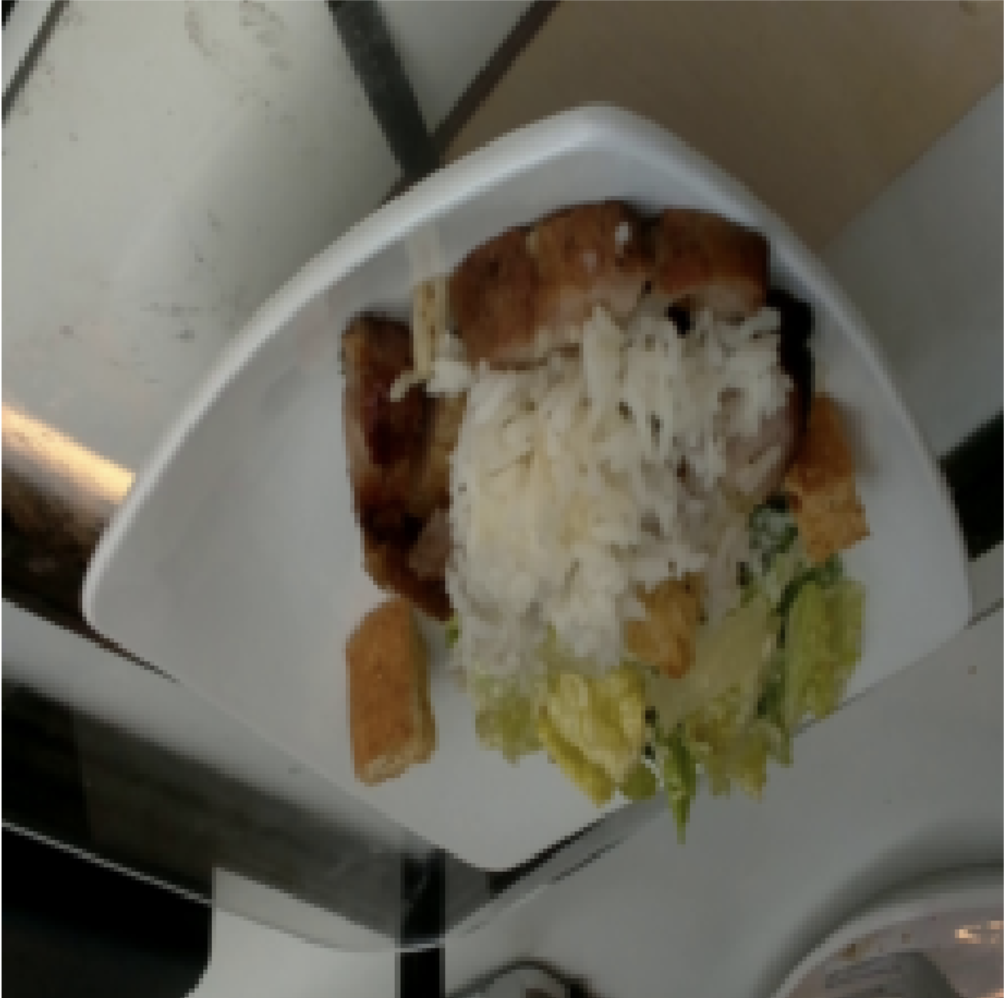
\includegraphics[width=4cm]{data/example-food-image} % Replace with actual image path
    };

    % Boxes for the diagram (shifted left)
    \node[draw, dashed, text width=4cm, align=left, inner sep=5pt] (per100g) at (0.5, 3.5) {
        \textbf{Per 100g:}\\
        Calories:\quad 174.0 kcal\\
        Fat:\quad 8.33 g\\
        Carbs:\quad 10.12 g\\
        Protein:\quad 14.73 g
    };

    \node[draw, dashed, text width=4cm, align=left, inner sep=5pt, below=5mm of per100g] (weight) {
        \textbf{Weight:}\quad 167.0 g
    };
    \node[scale=2] at ($(per100g.south)!.5!(weight.north)$) {$\times$};

    % Shifted closer (reduce spacing from 15mm → 8mm)
    \node[draw, text width=5.5cm, align=left, inner sep=5pt, right=8mm of $(per100g.east)!0.5!(weight.east)$] (total) {
    \textbf{Total:}\\
    Calories:\quad $174 \times 1.67 = 290.6$ kcal\\
    Fat:\quad $8.33 \times 1.67 = 13.9$ g\\
    Carbs:\quad $10.12 \times 1.67 = 16.9$ g\\
    Protein:\quad $14.73 \times 1.67 = 24.6$ g\\
    Weight:\quad 167.0 g
};

    % Arrows
    \draw[-Stealth, thick] (food_image.east) -- (per100g.west);
    \draw[-Stealth, thick] (food_image.east) -- (weight.west);
    \draw[-Stealth, thick] (per100g.east) -- (total.west);
    \draw[-Stealth, thick] (weight.east) -- (total.west);

\end{tikzpicture}


\vspace{1cm}
\begin{table}[h!]
\centering
\captionof{table}{Performance metrics of combined model: Weight est. * Per100g est.}
\label{tab:performance}
\begin{tabular}{lrrrrrr}
\toprule
\textbf{Nutrient} & \textbf{MAE} & \textbf{RMSE} & \textbf{R\textsuperscript{2}} & \textbf{MAE \%} & \textbf{Mean True} & \textbf{Mean Pred} \\
\midrule
Calories (abs) & 87.495 & 128.939 & 0.607 & \textbf{28.552} & 306.448 & 304.311 \\
Fat (abs) & 6.045 & 8.975 & 0.519 & \textbf{37.583} & 16.084 & 15.858 \\
Carbs (abs) & 7.760 & 12.154 & 0.449 & \textbf{37.008} & 20.969 & 21.700 \\
Protein (abs) & 7.588 & 11.938 & 0.686 & \textbf{34.080} & 22.265 & 20.851 \\
Weight (g) & 49.084 & 74.165 & 0.758 & \textbf{21.339} & 230.023 & 226.192 \\
\bottomrule
\end{tabular}
\end{table}


\vspace{1cm}
\begin{justify}
These results confirm that combining the two models together is indeed a reasonable approach. The pipeline demonstrates stable performance on the full dataset, predicting calories with a 28.552 MAE \%. These results set a solid foundation for further research and development on this topic, which we discuss in the next chapter.
\end{justify}


    \section{Conclusion and Future Work}
    Overall, the model we created is a robust approach for the challenging problem, achieving quite good results. Furthermore, this model can be trained on different cuisines and produce more consistent estimations than a human expert in some cases, who can have limited knowledge on rarer types of dishes.

    Another interesting point to consider is the cost of access to a professional nutritionist. For some people, nutrition is not necessarily a priority or might not even be considered an important health factor due to poor education or simple negligence. This is where solutions like FoodCNN might make a difference by allowing easy access to cheap and fast nutrition estimation to get insights into one's eating habits and how they could be improved upon.

    Some notable limitations we encountered and that could be improved upon in a future version of this project:

    \begin{itemize}
        \item Deep learning requires significant resources in terms of time and computational power that need to be taken into account.
        \item Segmentation could likely be improved by training a dedicated segmentation model on food data, which was not done due to time and complexity constraints.
        \item The Nutrition5k dataset was relatively small for the given task, and contained many small dishes. More food datasets could be used to allow the model to train on more examples.
    \end{itemize}


    
    \bibliographystyle{plain}
    \bibliography{bibliography}
    
\end{document}